\documentclass{article}
\usepackage[utf8]{inputenc}

% Default language is English. Enable Vietnamese only when needed.
\newif\ifusevietnamese
\usevietnamesefalse
% To use Vietnamese, uncomment the next line:
% \usevietnamesetrue

\ifusevietnamese
    \usepackage[T5]{fontenc}
    \usepackage{vntex}
    \usepackage[vietnamese,english]{babel}
\else
    \usepackage[T1]{fontenc}
    \usepackage[english]{babel}
\fi
\usepackage{lmodern}
\usepackage{fix-cm}

% Custom font size: between 13 pt and 14 pt
\usepackage{fontsize}
\changefontsize[18pt]{14pt}


% =========================================================
% PAGE LAYOUT
% =========================================================
\usepackage[
    a4paper,
    top=2.5cm,
    bottom=2.5cm,
    left=2.5cm,
    right=2.5cm
]{geometry}

\usepackage{setspace}
\setstretch{1.15}

\usepackage{indentfirst}
\setlength{\parindent}{1.25cm}
\setlength{\parskip}{0pt}


% =========================================================
% MATHEMATICS AND SYMBOLS
% =========================================================
\usepackage{amsmath}
\usepackage{mathtools}
\usepackage{bm}

% Units and scientific notation
\usepackage{siunitx}
\sisetup{
    detect-all,
    separate-uncertainty=true,
    per-mode=symbol
}

% Chemistry notation, if needed
\usepackage[version=4]{mhchem}

% =========================================================
% EQUATION SPACING
% =========================================================
\setlength{\abovedisplayskip}{6pt}
\setlength{\belowdisplayskip}{6pt}

\setlength{\abovedisplayshortskip}{3pt}
\setlength{\belowdisplayshortskip}{3pt}

% =========================================================
% FIGURES, TABLES, AND FLOATS
% =========================================================
\usepackage{graphicx}
\usepackage{subcaption}
\usepackage{float}
\usepackage{booktabs}
\usepackage{tabularx}
\usepackage{longtable}
\usepackage{array}
\usepackage{multirow}
\usepackage{adjustbox}
\usepackage{pdflscape}

\usepackage[
    font=small,
    labelfont=bf,
    labelsep=period
]{caption}

% Keep figures/tables inside sections if needed
\usepackage[section]{placeins}

% =========================================================
% DRAWING AND TITLE PAGE DECORATION
% =========================================================
\usepackage{tikz}
\usetikzlibrary{calc}
\usepackage{eso-pic}
\usetikzlibrary{positioning, arrows.meta}

% =========================================================
% LISTS
% =========================================================
\usepackage{enumitem}
\setlist[itemize]{topsep=3pt,itemsep=2pt}
\setlist[enumerate]{topsep=3pt,itemsep=2pt}

% =========================================================
% CODE LISTINGS
% =========================================================
\usepackage{xcolor}
\usepackage{listings}

\lstdefinestyle{pythonstyle}{
    language=Python,
    basicstyle=\ttfamily\small,
    breaklines=true,
    numbers=left,
    numberstyle=\tiny,
    frame=single,
    captionpos=b,
    showstringspaces=false
}

\lstdefinestyle{pseudostyle}{
    language={},
    basicstyle=\ttfamily\small,
    keywordstyle=\bfseries,
    commentstyle=\itshape,
    numbers=left,
    numberstyle=\tiny,
    stepnumber=1,
    frame=single,
    breaklines=true,
    breakatwhitespace=true,
    tabsize=4,
    showstringspaces=false,
    captionpos=b
}

% =========================================================
% BIBLIOGRAPHY
% =========================================================
% Option 1: modern bibliography system
\usepackage[numbers,sort&compress]{natbib}

% =========================================================
% APPENDICES, FOOTNOTES, COMMENTS
% =========================================================
\usepackage[toc]{appendix}
\usepackage[bottom]{footmisc}
\usepackage{comment}

% =========================================================
% HYPERLINKS AND CROSS-REFERENCES
% Load hyperref near the end
% =========================================================
\usepackage{hyperref}
\hypersetup{
    colorlinks=true,
    linkcolor=blue,
    citecolor=blue,
    urlcolor=cyan,
    filecolor=magenta,
    pdftitle={Incremental Nonlinear Dynamic Inversion Rate Control for a VTOL Quadplane UAV: Design and Software-in-the-Loop Evaluation},
    pdfauthor={Tran Anh Duy},
    bookmarksnumbered=true,
    bookmarksopen=true,
    bookmarksopenlevel=1,
    pdfpagemode=UseOutlines
}

\usepackage[nameinlink]{cleveref}

\newcommand{\HRule}{\rule{\linewidth}{0.5mm}}

\changefontsize[18pt]{13pt}

\begin{document}

% =========================================================
% TITLE PAGE
% =========================================================
\begin{titlepage}

\AddToShipoutPictureBG*{%
\begin{tikzpicture}[overlay,remember picture]
\draw[line width=3pt]
    ($(current page.north west) + (1cm,-1cm)$)
    rectangle
    ($(current page.south east) + (-1cm,1cm)$);
\draw[line width=1pt]
    ($(current page.north west) + (1.2cm,-1.2cm)$)
    rectangle
    ($(current page.south east) + (-1.2cm,1.2cm)$);
\end{tikzpicture}
}

\begin{center}

\vspace*{-0.8cm}

{\large\MakeUppercase{University of Science and Technology of Hanoi}}\\[0.3cm]
{\large\textbf{\MakeUppercase{Department of Space and Earth Sciences}}}\\[0.5cm]

% Replace with your logo file if available.
\ifdefined\IfFileExists
    \IfFileExists{usth.png}{
        \includegraphics[width=5cm]{usth.png}\\[0.2cm]
    }{
        \IfFileExists{./images/Logo.png}{
            
\includegraphics[width=5cm]{./images/Logo.png}\\[0.2cm]
        }{
            \vspace{0.5cm}
        }
    }
\fi
\vspace{0.3cm}
{\Large \textbf{BACHELOR THESIS}}\\[1.0cm]
{\large By}\\[0.2cm]
{\Large \textbf{Tran Anh Duy}}\\[0.8cm]

\HRule \\[0.4cm]
{\large \textbf{\MakeUppercase{
Development and Implementation of Autonomous Flight Control for a Vertical Take-Off and Landing Quadplane UAV
}}}\\[0.4cm]
\HRule \\[1.0cm]


\begin{tabular}{ll}
\textbf{\large Supervisors:} 
    & {\large Assoc. Prof. Pham Van Bach Ngoc  $^{1}$}\\[0.15cm]
    & {\large Dr. Nguyen Duc Hung $^{2}$}
\end{tabular}

\vspace{0.8cm}

{\large $^{1}$ \textit{Vietnam National Space Center, Vietnam}}\\[0.15cm]
{\large $^{2}$ \textit{University of Science and Technology of Hanoi, Vietnam}}\\[0.15cm]


\vfill

{\large Hanoi, 28 August 2026}

\end{center}
\end{titlepage}

\pagenumbering{roman}
\renewcommand{\contentsname}{Table of Contents}
\tableofcontents
\newpage

\section*{ACKNOWLEDGEMENTS}
\addcontentsline{toc}{section}{ACKNOWLEDGEMENTS}
I would like to express my deepest gratitude to my mentor and supervisor, Assoc. Prof. Pham Van Bach Ngoc, for his guidance, support, and encouragement throughout this project. He inspired me and gave me the chance to grow academically in his research group. This opportunity also brought me into contact with talented people and supported my professional growth.\\

I also thank my family for their support and encouragement throughout my studies. There were times I wanted to quit this project, but their support kept me going.\\

Throughout this project, my colleagues and friends have also provided incredible support, valuable feedback, and placed incredible trust in this project, for which I am deeply grateful.\\

Finally, I would like to express my heartfelt gratitude to my beloved, Le Ngoc Thuy Tien for being a constant source of motivation, support, and love throughout this project.\\
\newpage
\section*{LIST OF ABBREVIATIONS}
\addcontentsline{toc}{section}{LIST OF ABBREVIATIONS}
\noindent The abbreviations below are short for the following full terms.
\par\vspace{0.5\baselineskip}
\begin{longtable}{p{0.24\textwidth}p{0.68\textwidth}}
\textbf{Abbreviation}  \\
\midrule
UAV & Unmanned Aerial Vehicle \\
\midrule
VTOL & Vertical Take-Off and Landing \\
\midrule
INDI & Incremental Nonlinear Dynamic Inversion \\
\midrule
NDI & Nonlinear Dynamic Inversion \\
\midrule
PID & Proportional--Integral--Derivative \\
\midrule
SITL & Software-In-The-Loop \\
\midrule
TECS & Total Energy Control System \\
\midrule
EKF & Extended Kalman Filter \\
\midrule
IMU & Inertial Measurement Unit \\
\midrule
GPS & Global Positioning System \\
\midrule
MAVLink & Micro Air Vehicle Link \\
\midrule
CAD & Computer-Aided Design \\
\midrule
DOF & Degrees of Freedom \\
\midrule
ENU & East-North-Up \\
\midrule
FRD & Forward-Right-Down \\
\midrule
NED & North-East-Down \\
\midrule
MPC & Model Predictive Control \\
\midrule
SDF & Simulation Description Format \\
\midrule
SISO & Single-Input/Single-Output \\
\midrule
OpenVSP & Open Vehicle Sketch Pad \\
\midrule
CG & Centre of Gravity \\
\midrule
PSD & Power Spectral Density \\
\midrule
RMS & Root Mean Square \\
\midrule
RMSE & Root Mean Square Error \\
\end{longtable}
\setcounter{table}{0}% The uncaptained abbreviation list is not a numbered thesis table.
\newpage
\renewcommand{\listtablename}{LIST OF TABLES}
\listoftables
\renewcommand{\listfigurename}{LIST OF FIGURES}
\listoffigures
\newpage
\pagenumbering{arabic}

\section*{Abstract}
\addcontentsline{toc}{section}{Abstract}
This thesis investigates roll and pitch rate control for a vertical take-off and landing (VTOL) quadplane UAV with four lift motors and a pusher propeller. A physical prototype flew with ArduPilot PID control; the Incremental Nonlinear Dynamic Inversion (INDI) rate loop developed here was tested in Gazebo/ArduPilot software-in-the-loop (SITL).

The simulation uses aerodynamic coefficients from the built aircraft. This work derives a synchronized INDI law, estimates control effectiveness in SITL, and compares it with the configured PID baseline on the same simulated aircraft.

The lift motors and control surfaces share one INDI correction when both are active. Twelve SITL missions profiles were conducted, covering two paths and three wind conditions for each controller. In these single runs, INDI had lower take-off and transition pitch error; in a \SI{5}{\second} simulated pitch-torque test it held within \SI{0.1}{\degree}, versus up to \SI{2.5}{\degree} for PID. Wing-borne attitude and path results were mixed, with different lift-motor assist use and frequent saturation at \SI{9}{\meter\per\second}. The only real-flight log is mostly manual PID hover and cannot validate the simulated wing-borne behavior; its gyro vibration also highlights a difference between simulation and real flight. The comparison therefore describes this SITL model, not a demonstrated hardware advantage.

\noindent\textbf{Keywords}: quadplane, VTOL, UAV, INDI, PID, SITL.



\clearpage

\section{Introduction}
\label{sec:introduction}

\subsection{Motivation}
Aircraft that can take off and land vertically while also travelling efficiently in forward flight are useful for surveying, inspection, mapping, and other missions where a runway is unavailable.
A conventional multirotor drone could hover and maneuver precisely, but its propellers need to continuously generate downward thrust to support the aircraft, causing high energy consumption. On the other hand, a fixed-wing aircraft is efficient in forward flight, but it typically requires a runway or a launching system. A vertical take-off and landing (VTOL) vehicle combines these properties in one system.
This project focuses on the separate lift-cruise quadplane, whose lift motors and aerodynamic surfaces can act on the same axes during transition.

The combination is not simply the addition of a quadcopter and an aeroplane. In hover, the vehicle is controlled mainly through the independent thrust of the lift motors. In cruise, the wing produces most of the vertical force and the aircraft is controlled through aerodynamic surfaces and forward propulsion. During transition, both descriptions are active at the same time, and the controller must handle changes in pressure, actuator authority as lift is being created as the vehicle gains speed, trim, coupling, and available control margin (Section~\ref{sec:transition-corridor}). 

The combination of vertical take-off and efficient forward flight is useful for cargo missions where runway access is limited. For example, the manufacturer lists the Wingcopter 198, a tilt-rotor delivery aircraft, having a maximum range of \SI{94}{\kilo\meter} and a payload capacity of \SI{4.7}{\kilogram} \citep{wingcopter198}. These are manufacturer-stated specifications, rather than performance guaranteed for every route or operating condition. The example illustrates the potential of VTOL aircraft for moving useful payloads over distances that would be inefficient for a conventional multirotor.

There is also military interest in rapidly fielding small unmanned aircraft for logistics in locations that are difficult to reach by road or conventional aircraft. In 2024, U.S. Air Forces Central's Task Force 99, the Blue Horizons program, and Titan Dynamics assessed a software-designed, 3D-printed fixed-wing VTOL; a second prototype carried a mock first-aid package more than 30 miles to a simulated destination \citep{vermeulen2024taskforce99}.


\subsection{Research problem}
\label{sec:research-problem}

A quadplane combines vertical lift rotors with a traditional winged airframe. This lets it take off and land without a runway, but it makes attitude control harder in three ways.

First, the aircraft has two sets of effectors, and their authority changes with airspeed. In hover, roll and pitch are controlled by the lift motors alone. As the aircraft accelerates, the airflow over the wing and control surfaces grows and the surfaces gain authority, while the airflow through the lift rotors changes. During the transition, and whenever the lift motors assist the wing, both sets act on roll and pitch at the same time and their shares keep changing, as described in Section~\ref{sec:transition-corridor}.

Second, ArduPilot uses separate PID rate controllers for the motors and the surfaces, with airspeed scaling for the surfaces. Sustained disturbances are corrected by their integral action, which needs tracking error to build up.

Third, lift motors and control surfaces can produce roll and pitch moments together in transition. If each independently requested the full INDI correction, their moments would add and over-correct. The controller instead shares a correction between the two sets.

This thesis develops its rate-loop controller within ArduPilot rather than recreating a complete flight-control stack. ArduPilot's state estimator provides the state estimates needed by the controller, allowing the INDI controller and PID baseline to use the same estimator. The custom controller replaces only ArduPilot's rate-loop step (Section~\ref{sec:system-overview-methodology}); the existing arming, failsafe, and mode-transition mechanisms remain in place. Reusing these capabilities keeps the work focused on the rate-loop control law rather than on reimplementing estimation, flight modes, mixing, and logging.

For simulation, ArduPilot runs as Software-In-The-Loop (SITL), enabling the use of a desktop computer for testing and development. Gazebo supplies the vehicle physics, while a bridge carries simulated sensor data to SITL and actuator commands back to the simulator. Gazebo is used instead of SITL's internal physics model because ArduPilot provides an established Gazebo integration, and the model can represent the quadplane's rigid-body and aerodynamic behaviour (Section~\ref{sec:aero-methodology}) in a general-purpose simulator \citep{ardupilotdocs,ardupilotgazebo,gazebodocs}. Real and simulated flights also produce DataFlash logs that can be analysed with the same pipeline. This makes direct comparison possible, although it does not by itself establish that the simulated dynamics match the real aircraft.

Incremental Non-linear Dynamic Inversion (INDI) uses measured angular acceleration and control effectiveness instead of a complete aerodynamic model. Its performance still depends on measurement timing and effectiveness accuracy (Section~\ref{sec:indi-fw-implementation}).

The research problem therefore has two connected parts. First, the INDI law must be integrated into the high-rate body-rate loop, with one correction shared between the lift motors and the surfaces, while retaining ArduPilot's estimator, guidance, and safety mechanisms. Second, the simulation must be assessed against available real-flight data before simulated controller comparisons can be interpreted as evidence about the physical aircraft.   

\subsection{Scope and thesis organisation}
\label{sec:scope}
The work focuses on inner-loop roll and pitch rate control. Yaw, altitude, path planning, navigation, and state estimation remain with ArduPilot.

Section~\ref{sec:litreview} reviews rigid-body kinematics, cascaded PID, NDI, and the derivation and synchronization of INDI. Section~\ref{sec:methodology} describes the quadplane platform, the software architecture separating ArduPilot functions from custom INDI code, the simulation environment, and the verification methodology. Section~\ref{sec:results} presents simulation results, evaluates controller activity, and discusses limitations. Section~\ref{sec:conclusion} concludes and outlines future flight-testing steps.

\section{Objectives}
\label{sec:aims}
The primary objective of this thesis is to develop, integrate, and evaluate an Incremental Nonlinear Dynamic Inversion (INDI) attitude control law for a quadplane UAV. The specific aims are:
\begin{enumerate}
    \item \textbf{Implement synchronized INDI}: Develop roll and pitch rate control with matched feedback delays.
    \item \textbf{Integrate with ArduPilot}: Share the correction between lift motors and surfaces while retaining the stock PID fallback.
    \item \textbf{Evaluate in simulation}: Compare PID and INDI on the same Gazebo model and document limits on transferring results to hardware.
\end{enumerate}


\section{Literature Review}
\label{sec:litreview}

\subsection{Reference frames and rigid-body model}
\label{sec:sixdof}
The following reference frames and rigid-body model follow \citet{beardmclain2012} and provide the notation used later in this thesis.

\subsubsection{Reference frames}
Two frames are used throughout. The inertial frame $\mathcal{F}^{i}$ uses North-East-Down (NED) axes; the body frame $\mathcal{F}^{b}$ is centred on the aircraft and uses forward-right-down (FRD) axes. Gazebo's world coordinates are east-north-up, so the simulation interface converts between these conventions (Section~\ref{sec:platform-methodology}). The 3-2-1 yaw-pitch-roll Euler sequence relates the two frames through $R^{b}_{i}(\phi,\theta,\psi)$ \citep{beardmclain2012}.

\subsubsection{Twelve states, six degrees of freedom}
\label{sec:twelvestates}
A rigid body moving in three dimensions has six \emph{degrees of freedom} (DOF): translation along the body $x$, $y$, and $z$ axes, and rotation about those axes. A first-order model needs both a position-like value and its rate for each degree of freedom, giving twelve states:
\begin{itemize}
    \item \textbf{Translational (6 states):} position $(p_n,p_e,p_d)$ in $\mathcal{F}^i$, paired with body-frame velocity $\mathbf{v}=(u,v,w)$ in $\mathcal{F}^b$.
    \item \textbf{Rotational (6 states):} attitude, given by the Euler angles $(\phi,\theta,\psi)$, paired with body-frame angular rate $\boldsymbol{\omega}=(p,q,r)$ in $\mathcal{F}^b$.
\end{itemize}
This full state vector $\mathbf{x}=[p_n,p_e,p_d,u,v,w,\phi,\theta,\psi,p,q,r]^{T}$ is the twelve-state model used in \citep{beardmclain2012}. The kinematic pairing is
\begin{equation}
    \dot{\mathbf{p}}_{i}=R^{i}_{b}(\phi,\theta,\psi)\,\mathbf{v},\qquad
    \begin{bmatrix}\dot\phi\\\dot\theta\\\dot\psi\end{bmatrix}
    =\begin{bmatrix}1&\sin\phi\tan\theta&\cos\phi\tan\theta\\0&\cos\phi&-\sin\phi\\0&\sin\phi/\cos\theta&\cos\phi/\cos\theta\end{bmatrix}
    \begin{bmatrix}p\\q\\r\end{bmatrix},
    \label{eq:euler-kinematics}
\end{equation}
where $\mathbf{p}_i=(p_n,p_e,p_d)^T$. The Euler-rate transform is singular at $\theta=\pm90^{\circ}$ \citep{beardmclain2012}. Section~\ref{sec:rigidbody-dynamics} gives the force and moment equations for $\mathbf{v}$ and $\boldsymbol{\omega}$.

\subsubsection{Rigid-body dynamics}
\label{sec:rigidbody-dynamics}
Newton's second law, applied in the rotating body frame with the transport theorem $\left.\tfrac{d}{dt}\right|_i=\left.\tfrac{d}{dt}\right|_b+\boldsymbol{\omega}\times$, gives the translational and rotational equations of motion
\begin{equation}
    m\left(\dot{\mathbf{v}}+\boldsymbol{\omega}\times\mathbf{v}\right)=\mathbf{F}_{a}+\mathbf{F}_{p}+\mathbf{F}_{g},
    \label{eq:translation}
\end{equation}
\begin{equation}
    J\dot{\boldsymbol{\omega}}+\boldsymbol{\omega}\times(J\boldsymbol{\omega})=\boldsymbol{\tau}_{a}+\boldsymbol{\tau}_{p},
    \label{eq:rotation}
\end{equation}
where $\mathbf{F}_{a},\mathbf{F}_{p},\mathbf{F}_{g}$ and $\boldsymbol{\tau}_{a},\boldsymbol{\tau}_{p}$ are aerodynamic, propulsive, and gravitational contributions, and $\mathbf{v}$, $\boldsymbol{\omega}$ are body-frame velocity and angular rate \citep{beardmclain2012}. The $\boldsymbol{\omega}\times\mathbf{v}$ term accounts for using a rotating body frame. These equations support the simulation dynamics (Section~\ref{sec:platform-methodology}) and the control laws below.

% \subsubsection{How many variables control the body frame?}
% \label{sec:underactuation}
% Attitude, taken by itself, has three rotational degrees of freedom, and Eq.~\eqref{eq:rotation} needs in general three independent moments -- one about each body axis -- to control it fully. This is the three-axis roll/pitch/yaw command used by the rate loop implemented in this thesis.

% A narrower, frequently claim concerns not attitude but \emph{translational} force. A multirotor's only direct translational actuator is a scalar collective thrust along the body $z$-axis; there is no separate horizontal-thrust actuator. To redirect that thrust horizontally -- for example to correct horizontal position or track a velocity command -- the vehicle must tilt its thrust axis, and doing so only requires two of the three attitude angles, roll and pitch: they set the \emph{direction} of the body $z$-axis, which has only two degrees of freedom (a direction in three-dimensional space is a point on a sphere, parametrised by two angles), while yaw rotates the body about that same axis without changing its direction at all, and is therefore decoupled from thrust direction \citep{mahony2012multirotor}. This is why hovering multirotor control architectures command all three attitude angles, but use only two of them, $(\phi,\theta)$, as intermediate ``virtual controls'' generated by an outer position/velocity loop, while the third, $\psi$, is set independently, typically to hold or track heading \citep{mahony2012multirotor,beardmclain2012}. The body frame's \emph{orientation} therefore still needs three variables to be fully controlled; it is specifically the redirection of translational \emph{thrust} that needs only two of them, with the third left free.

In hover, the vehicle acts like a multirotor. It is underactuated: it has no direct horizontal thrusters. To move forward, backward, or sideways, it must tilt its body (roll and pitch) to point the lift-motor thrust vector in the desired direction. If attitude rate tracking is sluggish or unstable, horizontal position control degrades immediately. Furthermore, during transition to forward flight, dynamic pressure builds over the wings and control surfaces while lift-motor airflow changes dramatically. The inner loop must maintain stable attitude and damping across these aerodynamic shifts so the aircraft stays within its safe flight envelope.

\subsection{Attitude control architectures across vehicle classes}
\label{sec:architectures}

\subsubsection{Multirotor rate/attitude control}
A multirotor changes body moments by varying rotor thrust. Its usual cascade has an outer attitude loop producing desired body rates and an inner rate loop sending commands to the motor mixer. This structure also applies when the inner loop uses INDI \citep{lombaerts2019}.

\subsubsection{Fixed-wing attitude and energy control}
\label{sec:tecs}
A fixed-wing aircraft uses aerodynamic surfaces to control attitude. Their effectiveness increases with dynamic pressure, $\bar{q}=\tfrac{1}{2}\rho V^{2}$, so they have little authority at low airspeed. ArduPlane's Total Energy Control System (TECS) coordinates throttle and elevator with throttle changes the rate of energy gain or loss, while elevator determines how that energy is divided between airspeed and altitude \citep{lambregts1983tecs,ardupilotdocs}. During transition, lift-motor control gives way to these airspeed-dependent surfaces.

\subsubsection{The quadplane hybrid case and the transition corridor}
\label{sec:transition-corridor}
A quadplane uses lift motors for control at low speed and increasingly relies on wing lift and control surfaces as airspeed rises. This mixed regime is called the \emph{transition corridor} here. \citet{lombaerts2019} blend hover and aerodynamic \emph{models} across this regime; that blending is not itself a control law. Here the INDI correction for each axis is shared between motors and surfaces when both are active (Section~\ref{sec:indi-fw-implementation}).

\subsection{Nonlinear dynamic inversion and its main limitation}
\label{sec:ndi-theory}
Consider a nonlinear system:
\begin{equation}
    \dot{\mathbf{x}}=\mathbf{f}(\mathbf{x})+\mathbf{G}(\mathbf{x})\mathbf{u},\qquad \mathbf{y}=\mathbf{h}(\mathbf{x}),
    \label{eq:ndi-system}
\end{equation}
with state $\mathbf{x}$, control input $\mathbf{u}$, and output $\mathbf{y}$. Repeatedly differentiating an output $y_i$ eventually gives a derivative $y_i^{(r_i)}$ that contains $\mathbf{u}$. The first such derivative is the output's \emph{relative degree} \citep{lombaerts2019,steinertPart1_2025}. For all outputs, this gives
\begin{equation}
    \mathbf{y}^{(r)}(\mathbf{x})=\mathbf{l}(\mathbf{x})+\mathbf{M}(\mathbf{x})\,\mathbf{u},
    \label{eq:ndi-transformed}
\end{equation}
where $\mathbf{l}$ contains the parts of the dynamics that depend on the aircraft state, and $\mathbf{M}$ describes how the controls affect the output \citep{lombaerts2019}. If $\mathbf{M}$ can be inverted, or a pseudo-inverse can be used when there are extra actuators, the required command for the desired derivative $\boldsymbol{\nu}=\mathbf{y}^{(r)}_{\mathrm{des}}$ is
\begin{equation}
    \mathbf{u}_{\mathrm{cmd}}=\mathbf{M}^{-1}(\mathbf{x})\left[\boldsymbol{\nu}-\mathbf{l}(\mathbf{x})\right].
    \label{eq:ndi-law}
\end{equation}
In the ideal case, inserting Eq.~\eqref{eq:ndi-law} into Eq.~\eqref{eq:ndi-transformed} gives the requested output derivative. For rotational control, $\mathbf{l}$ includes the aerodynamic moments and $-\boldsymbol{\omega}\times(J\boldsymbol{\omega})$, while $\mathbf{M}(\mathbf{x})$ maps controls to angular acceleration \citep{lombaerts2019}.

NDI requires accurate estimates of both terms over the operating range; errors can reduce robustness \citep{snell1992,buffington1999}. INDI reduces this dependence by using a measured derivative in place of much of the state model \citep{steinertPart2_2025}. This is useful when the quadplane's aerodynamic model is approximate (Section~\ref{sec:aero-model-method}).

\subsection{Incremental nonlinear dynamic inversion}
\label{sec:indi-theory}

\subsubsection{Origins and the Taylor-series derivation}
\citet{smithberry2000} first flight-tested the incremental idea using a simplified NDI law developed from aircraft rotational dynamics by \citet{smith1998}. \citet{bacon2000} then gave a first-order Taylor-series derivation. This thesis uses that derivation because it matches the implemented rate loop (Section~\ref{sec:indi-implementation}). \citet{sieberling2010} later named the method Incremental Nonlinear Dynamic Inversion and showed that delay in angular-acceleration feedback is important. That delay was also important in this project (Section~\ref{sec:filtering-problem}).

Consider the system of Eq.~\eqref{eq:ndi-system} written for one differentiation as $\dot{\mathbf{x}}=\mathbf{F}(\mathbf{x},\mathbf{u})$. A first-order Taylor expansion of $\mathbf{F}$ around the operating point one sample in the past, $(\mathbf{x}_0,\mathbf{u}_0)=(\mathbf{x}(t-T_s),\mathbf{u}(t-T_s))$, gives
\begin{equation}
    \dot{\mathbf{x}}\approx\dot{\mathbf{x}}_0
    +\left.\frac{\partial\mathbf{F}}{\partial\mathbf{x}}\right|_{0}\!\!(\mathbf{x}-\mathbf{x}_0)
    +\left.\frac{\partial\mathbf{F}}{\partial\mathbf{u}}\right|_{0}\!\!(\mathbf{u}-\mathbf{u}_0),
    \label{eq:taylor}
\end{equation}
where $T_s$ is the control-loop sample time \citep{bacon2000,steinertPart1_2025}. Over one sample, INDI assumes that the input change affects $\dot{\mathbf{x}}$ more than the normal change in aircraft state. This compares the two Taylor terms in Eq.~\eqref{eq:taylor}, not $\mathbf{x}-\mathbf{x}_0$ and $\mathbf{u}-\mathbf{u}_0$ directly \citep{lombaerts2019,steinertPart1_2025}. This approximation requires the controller and actuators to act faster than the aircraft state changes. It was not independently checked for this quadplane. Dropping the state-change term and using $\left.\partial\mathbf{F}/\partial\mathbf{u}\right|_0=\mathbf{G}(\mathbf{x}_0)$ gives
\begin{equation}
    \begin{aligned}
        \dot{\mathbf{x}} &\approx \mathbf{F}(\mathbf{x}_0,\mathbf{u}_0)+\mathbf{G}(\mathbf{x}_0)(\mathbf{u}-\mathbf{u}_0)\\
        &=\dot{\mathbf{x}}_0+\mathbf{G}(\mathbf{x}_0)\,\Delta\mathbf{u},\qquad \Delta\mathbf{u}=\mathbf{u}-\mathbf{u}_0.
    \end{aligned}
    \label{eq:indi-taylor-simplified}
\end{equation}
Here, $\dot{\mathbf{x}}_0=\mathbf{F}(\mathbf{x}_0,\mathbf{u}_0)$ is the total measured state derivative at the previous sample. It includes the effect of the previous input, so it is not only the drift term $\mathbf{f}(\mathbf{x}_0)$. Setting $\boldsymbol{\nu}$ to the desired state derivative and solving Eq.~\eqref{eq:indi-taylor-simplified} for the command change gives
\begin{equation}
    \Delta\mathbf{u}=\mathbf{G}(\hat{\mathbf{x}}_0)^{-1}\left[\boldsymbol{\nu}-\hat{\dot{\mathbf{x}}}_0\right],\qquad
    \mathbf{u}=\hat{\mathbf{u}}_0+\Delta\mathbf{u},
    \label{eq:indi-general-law}
\end{equation}
Here, $\hat{\mathbf{u}}_0$ is the measured or estimated input from the previous sample; the hat shows that it is an estimate. In this controller, it comes from the command actually sent to the actuator and passes through the matching actuator and filter models \citep{bacon2000,steinertPart1_2025}. INDI adds $\Delta\mathbf{u}$ to this previous command. For example, a previous command of $0.30$ with an increment of $0.05$ gives a new command of $0.35$. Sending only $0.05$ would lose the existing trim. Unlike NDI, INDI only needs the local effectiveness $\mathbf{G}(\mathbf{x}_0)$. The measured derivative $\hat{\dot{\mathbf{x}}}_0$ replaces the other model terms \citep{steinertPart1_2025}. INDI is therefore called a \emph{sensor-based} method.

For rotational control, the state is the body angular rate, $\mathbf{x}=\boldsymbol{\omega}$, and $\boldsymbol{\nu}$ is the requested angular acceleration. The effectiveness $\mathbf{G}_{\omega}=\partial\dot{\boldsymbol{\omega}}/\partial\mathbf{u}$ tells how a command change changes angular acceleration \citep{steinertPart1_2025,lombaerts2019}.

This derivation matters for the implementation. INDI depends on the quality and timing of $\hat{\dot{\mathbf{x}}}_0$ and $\hat{\mathbf{u}}_0$ (Section~\ref{sec:synchronization-theory}). The time-scale separation behind Eq.~\eqref{eq:taylor} is an approximation, not independently verified for this airframe \citep{lombaerts2019,steinertPart1_2025}.

\subsubsection{Disturbance rejection: integral action versus incremental feedback}
\label{sec:pid-vs-indi-disturbance}
Consider one rotational axis with inertia $I$, control effectiveness $G$ (angular acceleration per unit command) and a constant disturbance moment $M_d$ applied at $t_0$:
\begin{equation}
    \dot\omega = G\,u + \frac{M_d}{I}.
    \label{eq:axis-disturbance}
\end{equation}
The angular rate is only affected by the input and the disturbance. Holding the rate requires $\dot\omega=0$, i.e.\ a command change $\Delta u^\ast=-M_d/(G I)$.

\textbf{PID.} With $e=\omega_{\mathrm{ref}}-\omega$ and $u=K_Pe+K_I\int e\,dt+K_D\dot e$, the integral term must provide $\Delta u^\ast$ once the error becomes zero. It changes at the rate $K_I e$, so it can build the required command only while an error exists. A sudden disturbance is therefore rejected gradually.

\textbf{INDI.} The disturbance enters the measured angular acceleration directly, $\dot\omega_f=G u_0+M_d/I$ (after the estimator filter). The law of Eq.~\eqref{eq:indi-general-law} then gives at the next step
\begin{equation}
    u = u_0+\frac{\nu-\dot\omega_f}{G} = \frac{\nu}{G}-\frac{M_d}{G I},
\end{equation}
which contains $\Delta u^\ast$ without waiting for rate error to build up in this simplified example. INDI needs measured acceleration, the previous applied command and the effectiveness estimate. Filter and actuator delays still matter \citep{steinertPart2_2025}. Section~\ref{sec:results-hover-test} shows the response to a constant simulated hover torque.

\subsubsection{Why INDI over PID, gain-scheduled NDI, or MPC}
\label{sec:why-indi}
The following points from the Steinert et al. survey and the tiltrotor study by \citet{lombaerts2019} explain why INDI was chosen for this project:
\begin{itemize}
    \item \textbf{Proportional Integral Derivative (PID).} ArduPilot already uses separate hover and fixed-wing PID loops and scales surface control with airspeed. INDI instead updates the command using measured angular acceleration and an effectiveness estimate; this comparison does not show that PID cannot be tuned to perform similarly \citep{lombaerts2019}.
    \item \textbf{Non-linear Dynamic Inversion (NDI).} INDI uses local effectiveness and measured acceleration instead of a full aircraft model. It can react to a disturbance before a rate error has built up \citep{steinertPart2_2025}.
    \item \textbf{Model Predictive Control (MPC).} MPC solves an optimisation problem over a future time horizon at every control step. It needs a prediction model and more computing power than was practical for this small, high-rate controller. The reviewed sources do not directly compare INDI and MPC, so this is an engineering choice for this project, not a result from those sources.
\end{itemize}
None of this makes INDI automatically better. Its dependence on effectiveness and acceleration measurement is discussed in the remainder of this section and in Section~\ref{sec:limitations}.

\subsection{Estimating angular acceleration and the synchronization problem}
\label{sec:synchronization-theory}
$\dot{\boldsymbol{\omega}}$ must be estimated from measured angular rate, for example by a backward difference. Differentiation amplifies sensor noise, so the estimate is filtered; filtering also introduces delay \citep{steinertPart2_2025}.

If acceleration feedback is filtered but applied-command feedback is not delayed similarly, INDI loses phase margin. \emph{Synchronization} filters the command feedback to match the acceleration path \citep{steinertPart2_2025}. The controller uses this for both motor and surface rate loops (Section~\ref{sec:indi-implementation}); matching it to real hardware remains untested.

Sampling and actuator dynamics also matter for INDI stability \citep{wang2019stability}. The first rate-loop implementation did not match feedback delays; Section~\ref{sec:filtering-problem} describes the correction made in SITL.

\section{Methodology}
\label{sec:methodology}
\label{sec:dev-workflow}
The work followed Fig.~\ref{fig:total-process}: build the aircraft, study its aerodynamics in OpenVSP, create a separate Gazebo model, and compare PID with INDI in SITL. The OpenVSP coefficients were not transferred directly into Gazebo. Only the PID-controlled prototype has flown; INDI has flown in simulation only.

\begin{figure}[H]
    \centering
    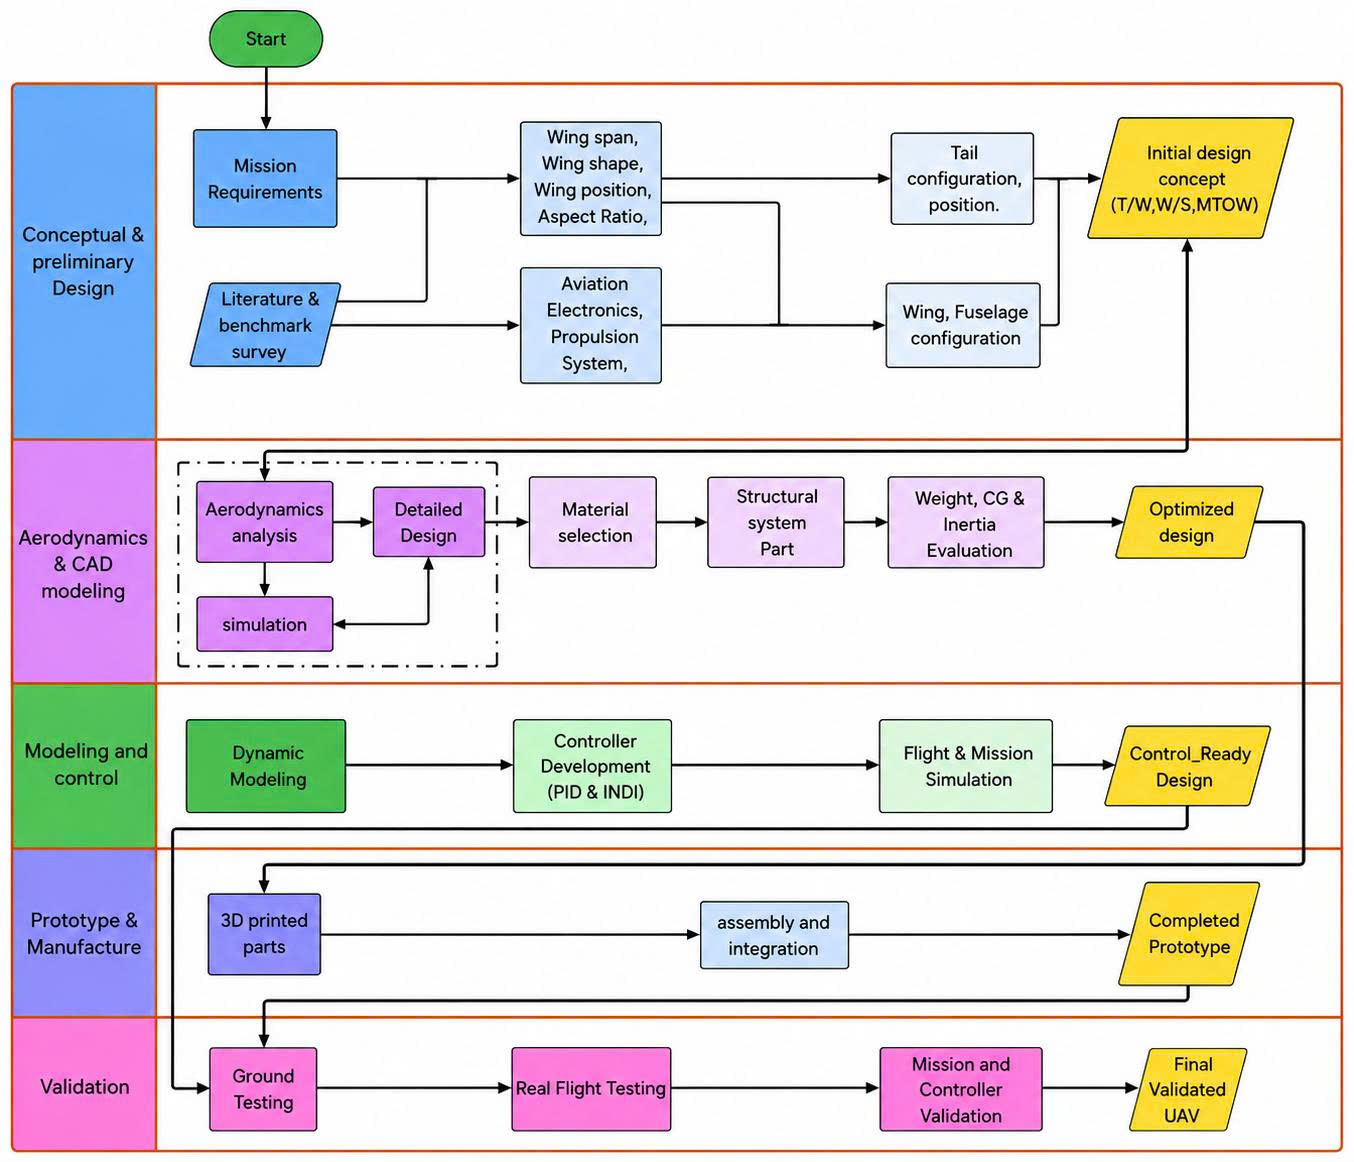
\includegraphics[width=\textwidth]{./images/Total process.jpeg}
    \caption{Overall project workflow, top-down design for prototyping and validation}
    \label{fig:total-process}
\end{figure}

\subsection{Aircraft, autopilot and simulator}
\label{sec:platform-methodology}
\label{sec:system-overview-methodology}
\label{sec:why-ardupilot}
\label{sec:sixdof-methodology}
The aircraft is a twin-boom quadplane (Fig.~\ref{fig:quadplane-concept}). Each boom holds two lift motors and ends at one of two vertical fins joined by a horizontal tail. A fuselage pusher provides cruise thrust. Lift motors control hover; the wing and surfaces become effective as airspeed builds. Figure~\ref{fig:stationary-bench} shows the assembled prototype, but does not provide motor bench-performance data.

\begin{figure}[H]
    \centering
    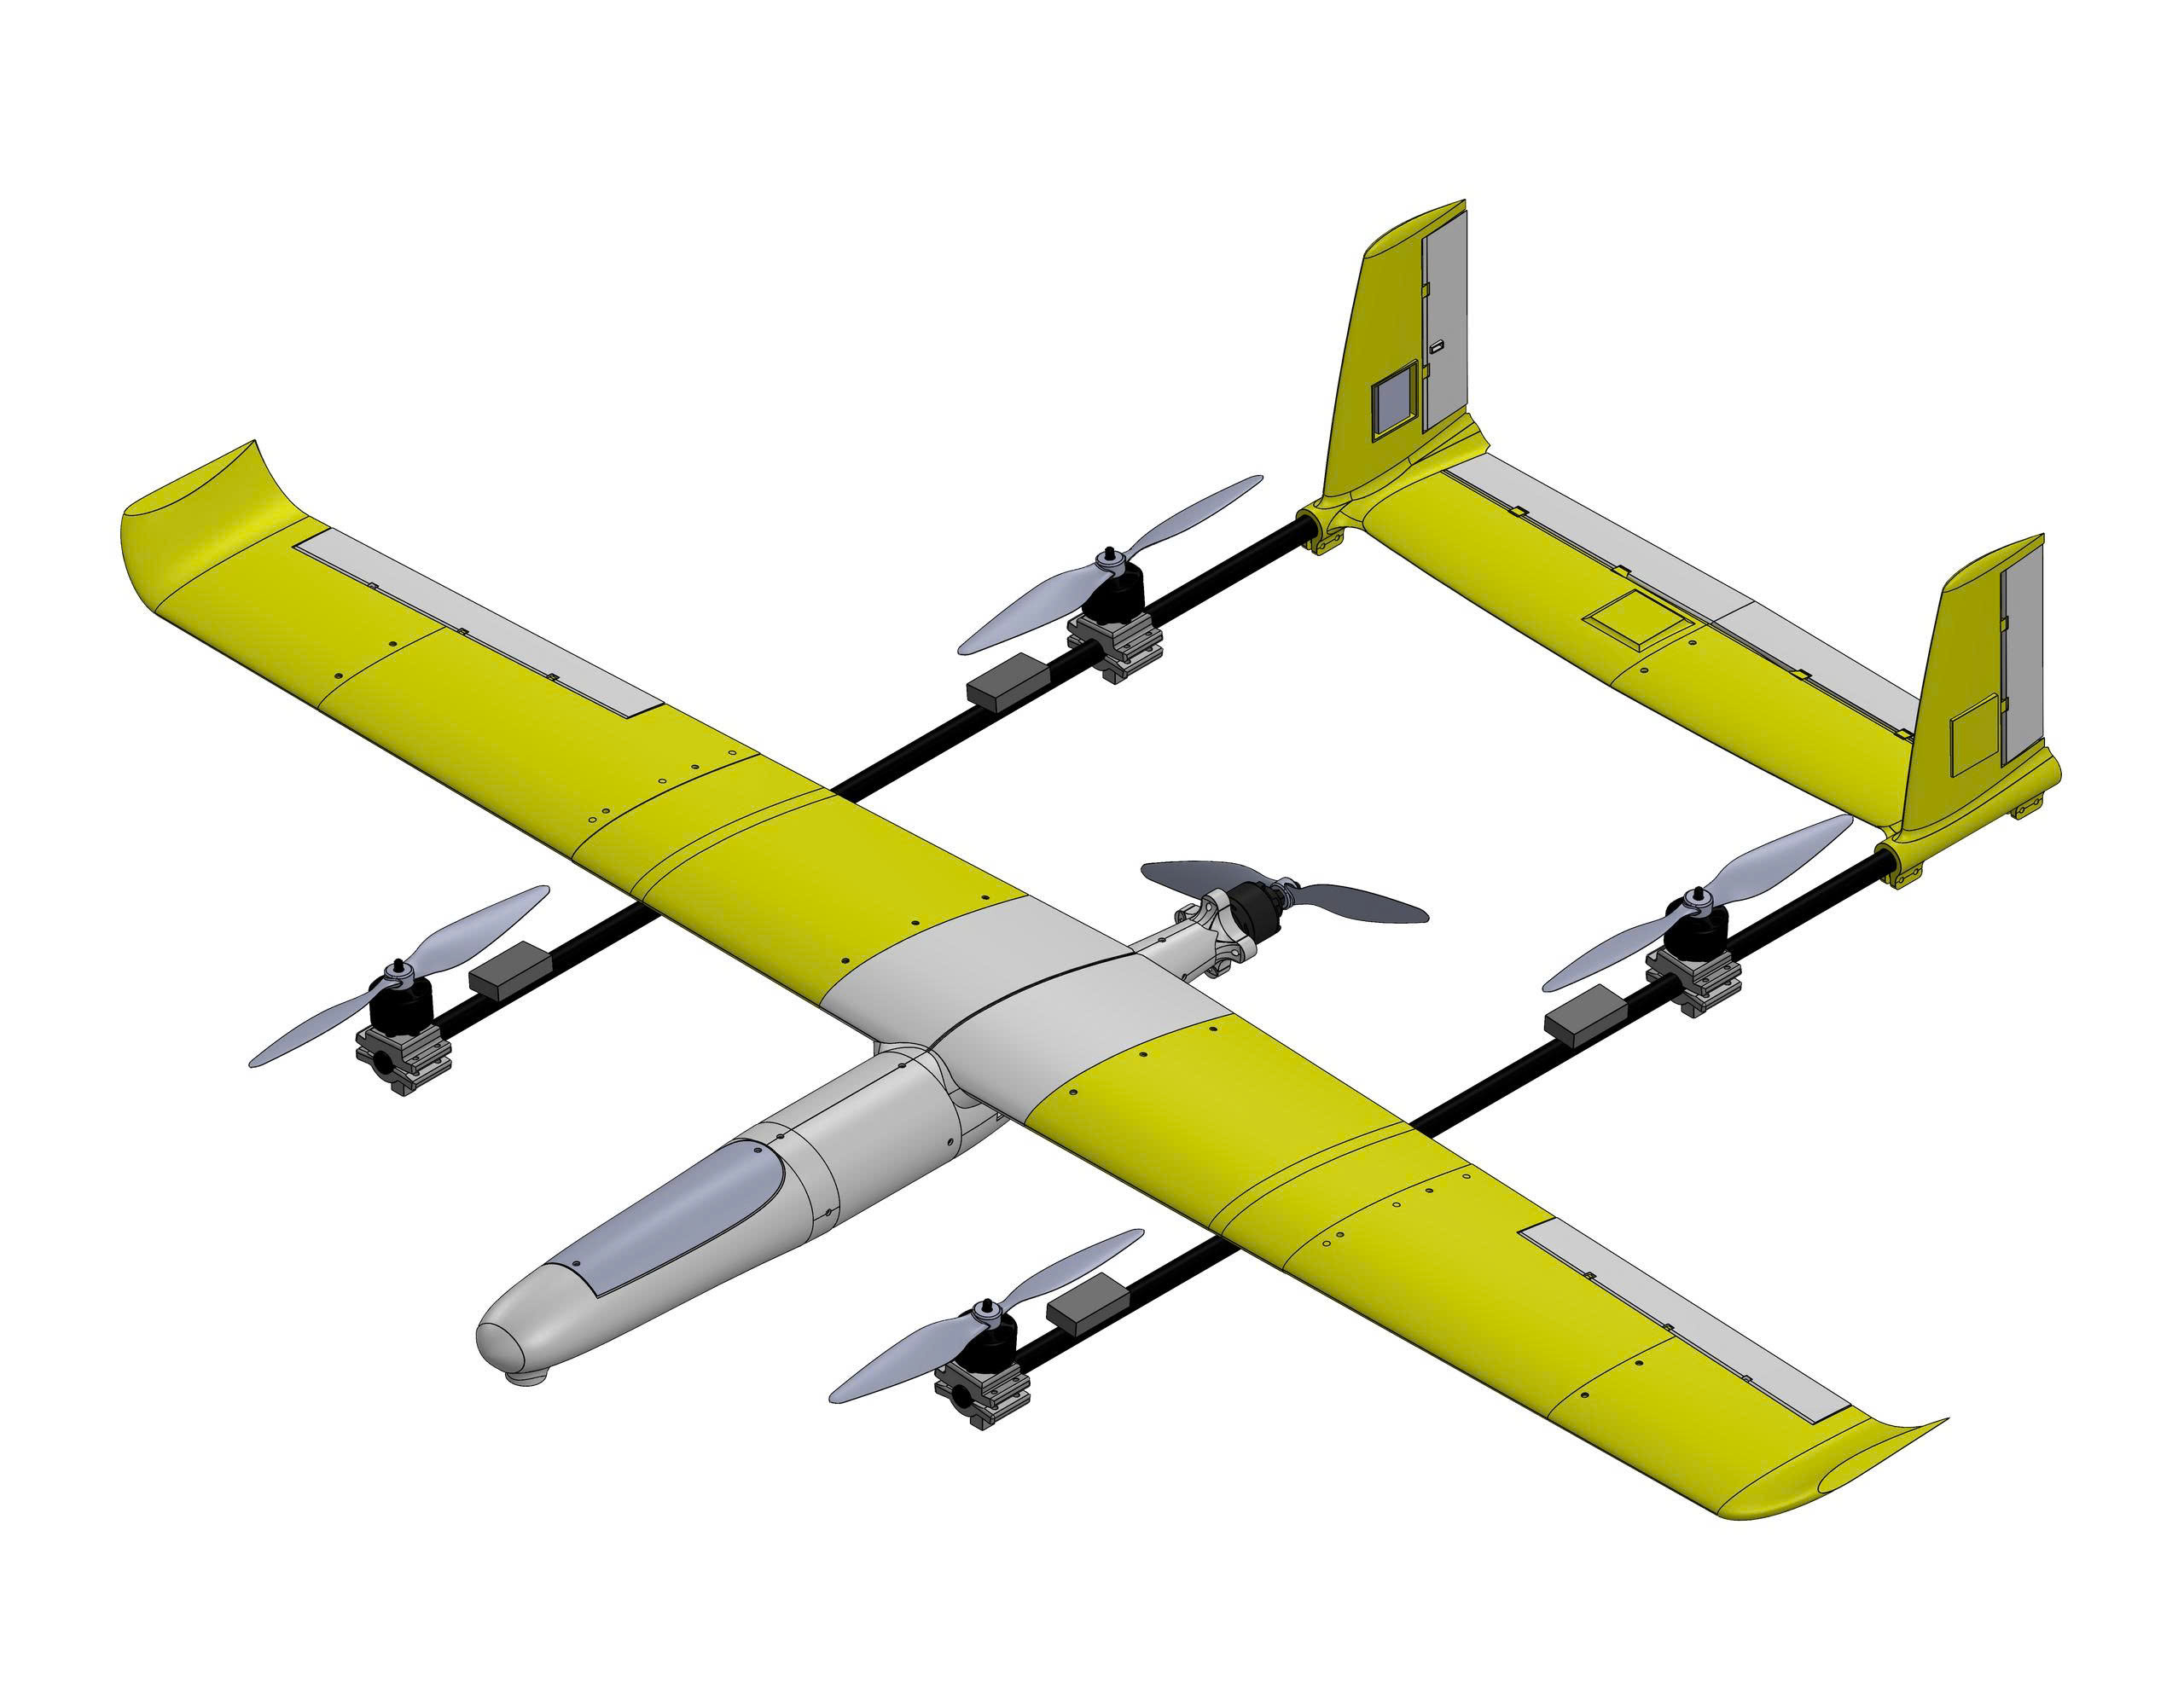
\includegraphics[width=0.75\textwidth]{./images/3D model.jpeg}
    \caption{CAD model of the quadplane: four lift motors, a pusher and a horizontal tail linking two fins.}
    \label{fig:quadplane-concept}
\end{figure}

The design geometry and CAD-derived mass properties of the aircraft are summarized in Table~\ref{tab:aircraft-specs}. The CAD values are taken from the authors' Version 3 SolidWorks assembly; they are design-model values, not independent measurements. Dimensioned top, front and left-side views are provided in Appendix~\ref{sec:appendix-build}.

\begin{table}[H]
\setlength{\tabcolsep}{4.5pt}\renewcommand{\arraystretch}{1.08}
    \centering
    \small
    \caption{Version 3 reference geometry and CAD-derived mass properties. Source: authors' SolidWorks CAD assembly.}
    \label{tab:aircraft-specs}
    \begin{tabularx}{\textwidth}{@{}>{\raggedright\arraybackslash}p{0.31\textwidth}>{\raggedright\arraybackslash}p{0.36\textwidth}>{\raggedright\arraybackslash}X@{}}
        \toprule
        Quantity & Reference value & Basis \\
        \midrule
        Mass; overall length
        & Approx. 3.1 kg design; 3.0346 kg CAD; 1.056 m
        & Nominal design and full-assembly CAD values \\
        \midrule

        Wingspan; wing area
        & 1.415 m; approx. 0.220 $\mathrm{m^2}$
        & 1.296 m flat panel plus two 59.57 mm winglet projections \\
        \midrule

        Wing section and incidence
        & NACA 4415; $4^\circ$
        & Nominal zero sweep and dihedral \\
        \midrule

        Wing chords
        & Root 0.180; panel tip 0.130; winglet-region tip 0.108 m
        & Three-station chord distribution \\
        \midrule

        Wing twist
        & $-3^\circ$ from $\eta=0.65$
        & Recorded geometric setting \\
        \midrule

        Horizontal tail
        & Span 0.460 m; area 0.042534 $\mathrm{m^2}$; arm 0.4876 m
        & Relative to recorded CG \\
        \midrule

        Vertical tails
        & Two fins, each 0.170 m high and 0.011572 $\mathrm{m^2}$
        & Area stated per fin \\
        \midrule

        Lift-motor arms
        & $a_f=0.290$, $a_r=0.300$, $d_y=0.245$ m
        & Nominal positions \\
        \midrule

        Full-assembly CAD CG
        & $(-0.32,20.70,-365.02)$ mm
        & Coordinates in the SolidWorks default frame \\
        \midrule

        Full-assembly CAD moments about CG
        & $I_{xx}=0.255360$, $I_{yy}=0.413556$, $I_{zz}=0.162775$
          ($\mathrm{kg\,m^2}$)
        & Full-assembly moments about the CG in SolidWorks default axes \\
        \bottomrule
    \end{tabularx}
\end{table}

The CAD inertias above use SolidWorks axes, not body FRD axes. The simulation's SDF base link instead has mass \SI{2.8}{\kilogram} and $I_{xx}=0.1399$, $I_{yy}=0.2138$, $I_{zz}=0.3502\,\mathrm{kg\,m^2}$ in its body axes (roll, pitch and yaw). These are base-link values, not a conversion of the full-assembly CAD inertias.

\begin{figure}[H]
    \centering
    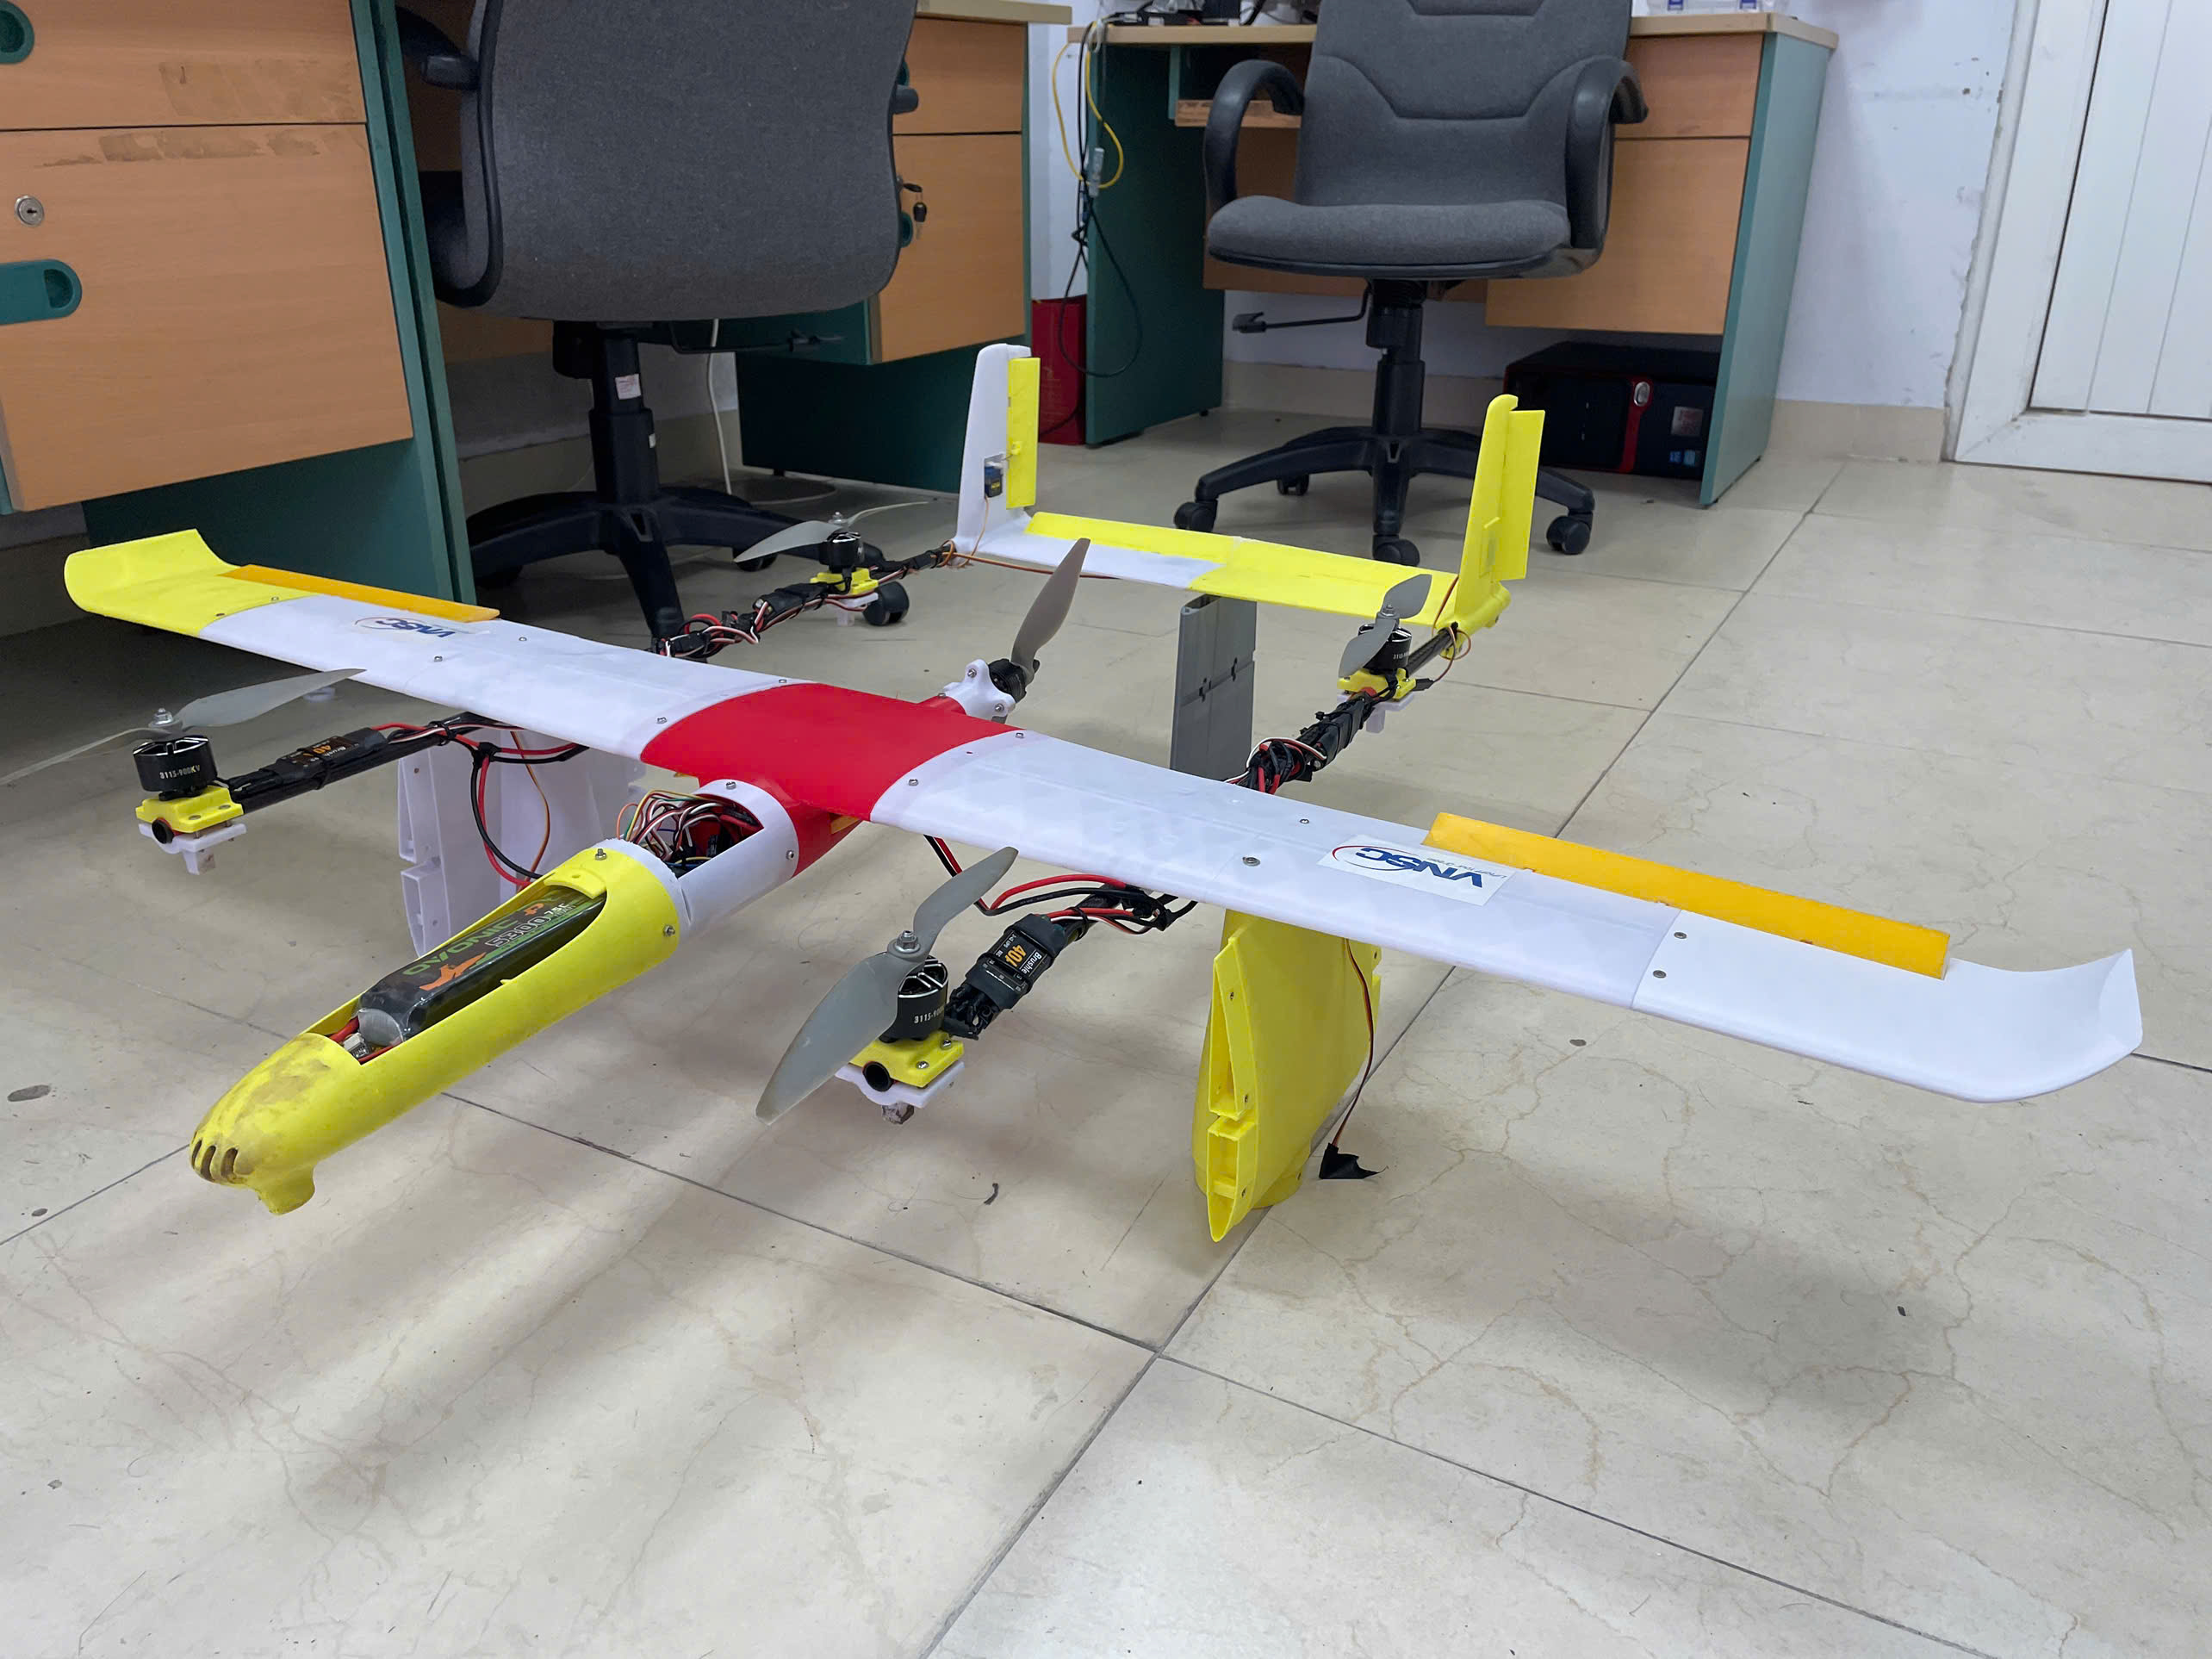
\includegraphics[width=0.85\textwidth]{./images/stationary bench.jpeg}
    \caption{Assembled prototype before flight; no motor thrust or response measurement is shown.}
    \label{fig:stationary-bench}
\end{figure}

\textbf{Autopilot.} ArduPilot was chosen because it is mature, open-source flight software that already supports quadplanes. It provides, unchanged:
\begin{itemize}
    \item sensor drivers and an extended Kalman filter that estimates attitude, rates, position and velocity;
    \item the outer attitude loop, which turns a desired attitude into a desired body rate;
    \item guidance, navigation, flight modes and the transition logic between hover and wing-borne flight;
    \item the mixer, which turns roll, pitch, yaw and throttle commands into motor and servo outputs;
    \item parameter storage and flight logging;
    \item the stock PID rate loop, which stays in the code as the fallback.
\end{itemize}
Only the roll and pitch rate-control step is replaced; yaw remains PID. The custom code also divides the INDI correction between motors and surfaces, while ArduPilot retains the mixer, outer attitude loop, navigation, altitude control and failsafes. Both runs use the same parameter set except for the INDI overlay. The PID gains were not independently retuned against the INDI margin target, so this is a comparison with the configured baseline, not with an optimally tuned PID.

\textbf{Simulator.} The same ArduPilot source is compiled for a desktop computer (software-in-the-loop, SITL) and connected to Gazebo, which computes the rigid-body motion and aerodynamic forces. A bridge passes motor and servo commands one way and IMU, barometer, GPS and airspeed data the other. Real and simulated flights produce the same log format, so one analysis pipeline reads both.

\textbf{Frames.} The body frame is forward-right-down, as in Section~\ref{sec:sixdof} and in ArduPilot. Gazebo uses east-north-up world axes, so the bridge converts between the two. A sign error here would reverse the aerodynamic and propulsive terms of Eqs.~\eqref{eq:translation}--\eqref{eq:rotation}, and the controller would look unstable when the fault is in the model interface.

\subsection{Aerodynamic model: from OpenVSP to Gazebo}
\label{sec:aero-model-method}
The CAD airframe was represented in OpenVSP \citep{openvspdocs} to estimate lift, drag and pitching moment. These results serve as a design reference, not the aerodynamic coefficients used by Gazebo. Lift and drag follow
\begin{equation}
    L=\tfrac{1}{2}\rho V^{2}SC_{L},\qquad D=\tfrac{1}{2}\rho V^{2}SC_{D}.
\end{equation}

Gazebo uses a lift-drag plugin. It represents each surface as one flat panel with a small set of parameters. Table~\ref{tab:liftdrag-params} in Appendix~\ref{sec:appendix-config} lists the main-wing values in the flown model and the available OpenVSP values. Appendix~\ref{sec:appendix-names} lists the matching SDF tag names. The wing, aileron sections, horizontal tail, elevator, vertical fins, rudders and winglets are each one panel, or a left and right pair. Below stall, the panel lift coefficient changes linearly with angle of attack:
\begin{equation}
    C_L = C_{L\alpha}\,(\alpha+\alpha_0) + k_\delta\,\delta ,
    \label{eq:gazebo-lift}
\end{equation}
where $\delta$ is a control-surface deflection. Gazebo does not read OpenVSP coefficients in flight. The simplified aileron and elevator panels, zero panel pitching-moment slopes, and nearly immobile simulated rudders limit the realism of wing-borne and transition results.

Each propeller is modelled the same way: two small lift-drag panels on a spinning link. ArduPilot commands the rotor speed, and the panels give a thrust that grows with the square of that speed.

\subsection{Rate controllers}
\label{sec:pid}
\label{sec:indi-implementation}
\textbf{PID baseline.} The configured ArduPilot loop compares the requested and measured body rates. It produces one normalised command for each axis:
\begin{equation}
    u(t)=K_Pe(t)+K_I\int_0^t e(\tau)\,d\tau+K_D\frac{de(t)}{dt},
    \label{eq:pid}
\end{equation}
where $e$ is the rate error. The mixer turns these commands and throttle into motor and servo outputs. The PID runs use the same firmware with the INDI switch off.

\textbf{INDI law.} INDI needs one value per axis: the control effectiveness $G$, or the change in angular acceleration caused by one unit of normalised command,
\begin{equation}
    \Delta\dot\omega = G\,\Delta u .
    \label{eq:effectiveness}
\end{equation}
Each axis (roll, pitch) then runs the same incremental law every control cycle:
\begin{align}
    \nu &= K\,(\omega_{\mathrm{ref}}-\omega) && \text{desired angular acceleration} \nonumber\\
    \dot\omega_f &= H\!\left(\tfrac{d\omega}{dt}\right) && \text{measured angular acceleration} \nonumber\\
    u_{0,f} &= H\!\left(F_g\!\left(A\,(u_{\mathrm{applied}})\right)\right) && \text{effector state, delayed to match} \nonumber\\
    u &= u_{0,f} + \frac{\nu-\dot\omega_f}{G} && \text{new command}
    \label{eq:diagonal-inversion}
\end{align}
The derivative is a backward difference of the gyro rate. $H$ is a low-pass filter with two equal poles at \SI{12.7}{\hertz}. $A$ is a model of the effector: a pure delay followed by a first-order lag. $F_g$ is a copy of the gyro filter that ArduPilot applies before the rate reaches the controller.

The applied command $u_{\mathrm{applied}}$ passes through the same three stages, $A$, $F_g$ and $H$. This makes its delay match the acceleration-feedback delay:
\begin{equation}
    u_{0,f} = H\,F_g\,A\;u_{\mathrm{applied}} .
    \label{eq:sync-fix}
\end{equation}
Filtering with $H$ alone was not enough; the loop limit-cycled until all three stages were matched (Section~\ref{sec:filtering-problem}). $u_{\mathrm{applied}}$ is what the mixer actually sent in the last cycle, recovered from the motor outputs, so saturation and mixer limits are included.

\textbf{Effectiveness.} For the lift motors, $G$ is a fixed value per axis, measured in simulated hover (Section~\ref{sec:results-identification}). For the control surfaces the moment grows with dynamic pressure, so
\begin{equation}
    G_s(V) = G_{s,\mathrm{ref}}\left(\frac{V}{V_{\mathrm{ref}}}\right)^{2},
    \label{eq:fw-indi-scaling}
\end{equation}
with $G_{s,\mathrm{ref}}$ referred to the reference airspeed $V_{\mathrm{ref}}=\SI{15}{\meter\per\second}$ and $V$ the measured airspeed. Yaw stays on the PID for both effector sets: its effectiveness could not be measured reliably (Section~\ref{sec:results-yaw}).

\subsection{Measuring control effectiveness}
\label{sec:identification-method}
Control effectiveness $G$ is the change in angular acceleration caused by a change in command (Eq.~\eqref{eq:effectiveness}). INDI needs this local response, not a model of the entire aircraft \citep{steinertPart1_2025}. Separate simulation flights measured $G$ before the PID--INDI comparison. One held a hover near \SI{40}{\meter}; another flew on the wing at three airspeeds. The stock PID kept the aircraft flying while a small test command was added in turn to motor roll, pitch and yaw, then to the ailerons and elevator. Each test lasted \SI{40}{\second}. The motor test swept from \SI{0.5}{\hertz} to \SI{20}{\hertz}; the surface test swept to \SI{15}{\hertz}.

The test command, total command and body rate were recorded. The change in body rate gives angular acceleration, so its response to the added test command estimates $G$. PID was also changing the command, so its output alone could not be used as the test input. The known test signal separates the aircraft response from PID corrections, as long as another disturbance is not linked to that signal \citep{ljung1999}. The analysis used frequencies above \SI{3}{\hertz} where the response followed the test signal clearly (coherence at least $0.6$). It then fitted $G$, a short lag and a delay. This removes weak data; it does not make the estimate exact.

Roll and pitch were tested separately for the lift motors and for the control surfaces, giving one motor and one surface effectiveness per axis. Surface effectiveness increases with airspeed, so the values are compared at \SI{15}{\meter\per\second} and scaled with $V^2$ as in Eq.~\eqref{eq:fw-indi-scaling}. When both sets act on an axis, their effects add as described in Section~\ref{sec:indi-fw-implementation}. Possible effects between different axes were not measured, and the small test responses may not describe large or saturated commands. The measured values and their limitations are discussed in Section~\ref{sec:results-identification}.

\subsection{Motors and surfaces share one INDI correction}
\label{sec:indi-fw-implementation}
A quadplane has two sets of roll and pitch effectors: lift motors and control surfaces. Both may act during hover, transition and assisted wing-borne flight. Two independent full INDI corrections would double the ideal acceleration change; the implementation shares a correction instead.

This is not a separate published quadplane INDI law. It combines the INDI effectiveness relation in Eq.~\eqref{eq:effectiveness} \citep{bacon2000,steinertPart1_2025} with standard pseudo-inverse control allocation \citep{johansenfossen2013}. The method assumes that motor and surface moments add on one axis and that their normalised commands have equal importance.

\textbf{Two independent INDI.} With motor effectiveness $G_m$ and surface effectiveness $G_s$, two loops using the same acceleration error $\nu-\dot\omega_f$ give, from Eq.~\eqref{eq:effectiveness},
\begin{equation}
    \Delta u_m = \frac{\nu-\dot\omega_f}{G_m}, \qquad \Delta u_s = \frac{\nu-\dot\omega_f}{G_s},
    \label{eq:indi-independent-increments}
\end{equation}
This is the command-change part of Eq.~\eqref{eq:diagonal-inversion} for each loop \citep{bacon2000,steinertPart1_2025}. Using these commands in the effectiveness equation gives
\begin{equation}
    \Delta\dot\omega = G_m\,\Delta u_m + G_s\,\Delta u_s = 2\,(\nu-\dot\omega_f).
    \label{eq:indi-double-correction}
\end{equation}
Equation~\eqref{eq:indi-double-correction} follows directly from the cited INDI effectiveness relation and the assumption that the two incremental moments add. It shows that two full corrections request twice the intended acceleration change. This holds whatever the size of $G_s$: a weak surface simply needs a larger command. The loop model in Table~\ref{tab:joint-margins} gives smaller, but still positive, margins for independent laws. That case was analysed but not flown.

\textbf{One correction, split between the effectors.} The single relation for one axis is
\begin{equation}
    G_m\,\Delta u_m + G_s\,\Delta u_s = \nu-\dot\omega_f ,
    \label{eq:indi-shared-constraint}
\end{equation}
This is Eq.~\eqref{eq:effectiveness} with two effectors. There are two commands but only one requested acceleration. The standard pseudo-inverse method chooses the smallest pair of commands that produces that acceleration: $\Delta\mathbf{u}=\mathbf{G}^{T}(\mathbf{G}\mathbf{G}^{T})^{-1}(\nu-\dot\omega_f)$, where $\mathbf{G}=[G_m\;G_s]$ \citep{johansenfossen2013}. For this two-effector case, it gives
\begin{equation}
    \Delta u_i = \frac{G_i\,(\nu-\dot\omega_f)}{G_m^2+G_s^2}, \qquad i\in\{m,s\}.
    \label{eq:indi-allocation}
\end{equation}
Equation~\eqref{eq:indi-allocation} is the two-effector form of the cited allocation method, applied to the INDI correction. It is not a new method. Without saturation, it gives the one requested acceleration in Eq.~\eqref{eq:indi-shared-constraint}. The shares $G_i^2/(G_m^2+G_s^2)$ apply to the separately normalised commands; they do not describe energy efficiency. This implementation does not redistribute a correction after an effector reaches its limit. When one set stops, the other receives the full correction.

\textbf{Surface effectiveness.} $G_s$ follows Eq.~\eqref{eq:fw-indi-scaling} using ArduPilot's airspeed estimate. The implementation sets it to zero at or below half the configured minimum airspeed, \SI{7}{\meter\per\second}. This is a controller gate, not a measured aerodynamic threshold. In calm hover the surfaces remain on PID; in \SI{9}{\meter\per\second} wind their estimated share is about \SI{1}{\percent}.

\textbf{Margins.} In the discrete SITL loop model at \SI{333}{\hertz}, the shared correction retains about \SI{9}{\decibel} gain margin and \ang{46} phase margin. Two independent full corrections leave about \SI{3.5}{\decibel} and \ang{27} when surfaces engage (Table~\ref{tab:joint-margins}). These are model predictions, not results from an independent-law flight.

\begin{table}[H]
\centering
\caption{Roll-axis margins with both effector sets on INDI: the shared correction keeps the single-loop margins, independent laws lose about \SI{5.5}{\decibel}.}
\label{tab:joint-margins}
\begin{tabular}{rrrcc}
\hline
Airspeed & $G_s$ & Surface share & Shared correction & Independent laws \\
{[\si{\meter\per\second}]} & [\si{\radian\per\second\squared}] & $G_s^2/\sum G^2$ & GM [\si{\decibel}] / PM [\si{\degree}] & GM [\si{\decibel}] / PM [\si{\degree}] \\
\hline
0--7 & 0    & \SI{0}{\percent}    & 9.0 / 45.9 & 9.0 / 45.9 \\
\hline
9    & 6.0  & \SI{1.1}{\percent}  & 9.0 / 45.8 & 3.5 / 26.6 \\
\hline
14   & 14.5 & \SI{6.2}{\percent}  & 9.1 / 45.8 & 3.5 / 26.6 \\
\hline
17   & 21.5 & \SI{12.5}{\percent} & 9.2 / 45.8 & 3.5 / 26.6 \\
\hline
22   & 35.9 & \SI{28.6}{\percent} & 9.4 / 45.8 & 3.5 / 26.6 \\
\hline
\end{tabular}
\end{table}

\textbf{Which loop runs.} Listing~\ref{lst:ownership} is the rule evaluated every control cycle. INDI is used wherever an effector has a known effectiveness; the stock PID is the last fallback.

\begin{lstlisting}[style=pseudostyle, caption={INDI and PID per effector set, every control cycle.}, label={lst:ownership}]
lift motors running (hover, transition, assist):
    roll, pitch -> INDI with share G_m^2 / (G_m^2 + G_s^2)
surfaces (every phase):
    if airspeed > 7 m/s:
        roll, pitch -> INDI with share G_s^2 / (G_m^2 + G_s^2)
                       (G_m = 0 once the lift motors are off)
    else:
        roll, pitch -> stock PID
yaw -> stock PID, always
fallback to stock PID: INDI switched off, G = 0, or motors not spun up
\end{lstlisting}

The motor and surface updates run in separate parts of ArduPilot. Each uses the other loop's latest $G$ in the shared denominator and ignores reports older than \SI{10}{\milli\second}. The sharing is approximate because there is no single simultaneous allocator, and the loops use different rate gains. The results include times when both updates were active, but not two independent full corrections.

\subsection{Simulation set-up and flight profiles}
\label{sec:sim-to-real}
\label{sec:mission-profile}
Each case uses fresh autopilot memory and archives its log, parameters, world file and mission status. Two missions were flown (Table~\ref{tab:profiles}). The runner removes waypoints too close to a landing point; path plots use the resulting mission, not the unmodified plan.

\textbf{Square circuit.} Vertical take-off to \SI{35}{\meter}, a closed square of about \SI{250}{\meter} per side, and a vertical landing at the take-off point. One circuit contains every phase: hover, forward transition, wing-borne flight with four \ang{90} turns, back transition, and hover. Because the aircraft flies all four headings, one steady wind is a crosswind, headwind, opposite crosswind and tailwind in turn, all in one log.

\textbf{Zigzag.} Five parallel \SI{500}{\meter} legs, \SI{100}{\meter} apart at \SI{35}{\meter} altitude, create four tight turnarounds. The landing is about \SI{765}{\meter} from take-off. The runner removes the final two waypoints because they are too close to this landing point, so the flown last leg runs straight to landing.

\begin{table}[H]
\centering
\caption{The two flight profiles.}
\label{tab:profiles}
\begin{tabular}{lcc}
\hline
 & Square circuit & Zigzag \\
\hline
Legs & 4 $\times$ \SI{250}{\meter} & 5 $\times$ \SI{500}{\meter}, \SI{100}{\meter} apart \\
\hline
Turns & 4 $\times$ \ang{90} & 4 $\times$ \ang{180} (each two \ang{90}) \\
\hline
Altitude & \SI{35}{\meter} & \SI{35}{\meter} \\
\hline
Landing & at take-off point & far end, \SI{765}{\meter} away \\
\hline
Tests & all phases, all wind headings & repeated quick turns \\
\hline
\end{tabular}
\end{table}

\textbf{Airspeed settings.} A quadplane switches its lift motors on to help the wing (``assist'') whenever it believes the airspeed is too low. In the earlier campaign a setting forced this help on for the whole flight, and the speed limits were above what the aircraft could reach. The ``fixed-wing'' part of every earlier run was therefore flown with the lift motors running, and no surface controller was ever tested on the wing alone. The speed limits were re-set from the model's stall speed (Section~\ref{sec:aero-methodology}):
\begin{itemize}
    \item stall speed \SI{12}{\meter\per\second};
    \item minimum airspeed \SI{14}{\meter\per\second};
    \item lift-motor assist only below \SI{13}{\meter\per\second}, as a low-speed safety net, and the forced-assist setting cleared;
    \item cruise \SI{17}{\meter\per\second}, which the model holds.
\end{itemize}

\subsection{Wind and disturbance injection}
\label{sec:wind-injection}
Wind is set in the Gazebo world file as one steady vector per case. The WindEffects plugin also adds small variations to the world-wind velocity (\SI{0.3}{\meter\per\second} horizontal magnitude, \SI{0.02}{\radian} direction and \SI{0.05}{\meter\per\second} vertical standard deviations). Its direct body-force approximation is set to zero: wind instead affects the lift-drag panels and ArduPilot's airspeed estimate. Two checks are relevant:
\begin{enumerate}
    \item \emph{The aerodynamics see the wind.} Each lift-drag panel computes its own air-relative velocity from the world wind.
    \item \emph{The autopilot sees the same wind.} The bridge now sends the wind vector to ArduPilot, so its airspeed is air-relative and not ground speed.
\end{enumerate}
The crosswind crab-angle check supports this wind path (Section~\ref{sec:results-wind}).

The disturbance is a torque applied directly to the airframe, not an aerodynamic gust. The chosen scaling $M=\tfrac12\rho u^2 S\,b/4$ uses $S=\SI{0.204}{\meter\squared}$ and $b=\SI{1.296}{\meter}$ to set \SI{1.44}{\newton\meter} at \SI{6}{\meter\per\second} and \SI{3.24}{\newton\meter} at \SI{9}{\meter\per\second}; it is a test convention, not a measured gust moment.

\subsection{Test configuration and scenarios}
\label{sec:test-scenarios}
Each profile is flown by both controllers in three conditions (Table~\ref{tab:test-matrix}, with wind also given as a fraction of the \SI{17}{\meter\per\second} cruise airspeed): twelve runs, one seed each, all with the calibrated IMU noise of Section~\ref{sec:results-wind}. Every case uses the same aircraft model and mission; PID and INDI differ only in the INDI parameter block. Condition 1 is the calm baseline. Conditions 2 and 3 add moment pulses on top of the wind (Table~\ref{tab:disturbance-points}): each window is a roll pulse, \SI{2}{\second} rest, then a pitch pulse, each \SI{1}{\second} long. Times are on the vehicle clock and positions come from the planned path, so PID and INDI receive the pulses at the same point of the mission; a window that triggers while the previous one is still running waits for it to finish.

\begin{table}[H]
\centering
\caption{Test conditions, each flown by PID and INDI on both profiles.}
\label{tab:test-matrix}
\begin{tabular}{lcccc}
\hline
Condition & Wind [\si{\meter\per\second}] & Wind [\si{\kilo\meter\per\hour}] & Fraction of cruise & Moment pulse \\
\hline
1 calm      & 0 & 0    & ---               & none \\
\hline
2 moderate  & 6 & 21.6 & \SI{35}{\percent} & \SI{1.44}{\newton\meter} \\
\hline
3 strong    & 9 & 32.4 & \SI{53}{\percent} & \SI{3.24}{\newton\meter} \\
\hline
\end{tabular}
\end{table}

\begin{table}[H]
\centering
\caption{Moment-pulse windows in conditions 2 and 3, at the same mission points for PID and INDI.}
\label{tab:disturbance-points}
\begin{tabular}{p{0.2\textwidth}p{0.52\textwidth}p{0.16\textwidth}}
\hline
Window & Starts & Square / zigzag \\
\hline
Take-off hover & \SI{4}{\second} after take-off begins & 1 / 1 \\
\hline
Transition & \SI{3}{\second} after the transition starts & 1 / 1 \\
\hline
Corner & when a waypoint where the path turns more than \ang{45} is reached & 3 / 8 \\
\hline
Leg midpoint & half way along every leg of at least \SI{200}{\meter}: \SI{125}{\meter} into a square side, \SI{250}{\meter} into a zigzag leg & 4 / 5 \\
\hline
Landing hover & \SI{5}{\second} after the landing descent starts & 1 / 1 \\
\hline
\multicolumn{3}{p{0.92\textwidth}}{Corner and midpoint windows fire only in wing-borne flight, after the transition is done and before the back-transition starts; a point reached outside that interval is skipped and logged.} \\
\hline
\end{tabular}
\end{table}

A separate hover torque test checks that INDI, and not the fallback PID, is in control: the aircraft holds position over the origin in the position-hold hover mode while a constant roll and then pitch torque is applied for \SI{5}{\second} each (Section~\ref{sec:results-hover-test}). The resulting three-dimensional hover trajectories are provided in Appendix~\ref{sec:appendix-results} (Fig.~\ref{fig:hover-torque-path3d}).

Vertical guidance and altitude control remain in ArduPilot in both configurations: its QuadPlane controller is used in VTOL phases, while TECS controls height and airspeed in wing-borne flight \citep{ardupilottransitions,ardupilottecs}. The INDI build changes only the roll and pitch rate paths. For analysis, phases are delimited from the logged autopilot status messages, beginning with ``Transition started'' and ``Transition done'' and ending with the back-transition and landing messages.

\subsection{Metrics and analysis procedure}
\label{sec:metrics}
For $N$ logged error samples $e_k$ in each phase, the tracking error is
\begin{equation}
    \mathrm{RMSE}=\sqrt{\frac{1}{N}\sum_{k=1}^{N} e_k^2}.
    \label{eq:rmse}
\end{equation}
It is applied to the attitude error (desired minus actual) and to the rate error (rate target minus measured rate). For each pulse, the peak change of the attitude error in the \SI{3}{\second} after its start is taken, relative to its mean over the second before. Other measures are the crab angle in crosswind, the time with lift-motor assist, and the share of time each axis runs INDI.

\textbf{Gyro-noise band RMS.} For the hover-noise comparison, the sampled gyro rate is differentiated to obtain angular acceleration, and its power spectral density (PSD) $S_{\dot\omega}(f)$ is estimated from the frequency spectrum. To estimate the noise after the physical aircraft's \SI{42}{\hertz} gyro filter, the PSD is weighted by the squared magnitude of its filter response $|H_{42}(f)|^2$. The noise power in the \SIrange{25}{90}{\hertz} band is the area under this filtered PSD; its square root gives RMS angular-acceleration noise:
\begin{equation}
    \sigma_{25\text{--}90}=\sqrt{\int_{25\,\mathrm{Hz}}^{90\,\mathrm{Hz}} S_{\dot\omega}(f)\,|H_{42}(f)|^2\,df}.
    \label{eq:gyro-band-rms}
\end{equation}
For the unfiltered value $H_{42}=1$. With discrete frequency bins, the integral is evaluated as a sum of PSD values multiplied by their frequency-bin width before taking the square root; the bin amplitudes themselves are not added. The simulated value is obtained from its own logged gyro-filter setting, rather than applying the aircraft's \SI{42}{\hertz} filter to simulation data.

\textbf{Path error.} The desired path is the planned polyline from the take-off point through the waypoints to the landing point, at the planned altitude, read from the same mission file the aircraft flew. For every logged position the nearest point of that polyline is found in the horizontal plane. The error vector from that point to the aircraft gives
\begin{equation}
    e_x = n - n_{\mathrm{path}}, \qquad e_y = e - e_{\mathrm{path}}, \qquad e_z = h - h_{\mathrm{path}},
    \label{eq:path-error}
\end{equation}
with $n$ and $e$ the north and east position and $h$ the height above the take-off point; the signed cross-track error is its component across the leg, positive to the right. The path has no timing, so there is no along-track error. $e_z$ is defined only in the transition, wing-borne and back-transition phases, where the plan holds an altitude. Statistics are reported per phase and, for wing-borne flight, also on straight legs only, leaving out points within \SI{60}{\meter} of a waypoint, which separates leg tracking from the corner cut set by the turn radius.

\textbf{Common clock.} Pulses occur at mission points but at different times in PID and INDI runs. In comparison plots, corresponding pulse windows are aligned; time between windows is stretched or compressed and must not be read as the actual flight duration.

\textbf{Saturation.} A lift motor is at a limit when its output is at the minimum or maximum spin setting while the motors run; a surface is saturated at \SI{98}{\percent} of its travel. For each pulse the analysis records whether any lift motor was at a limit, or the surface of the pulsed axis saturated, within \SI{2}{\second} of the pulse start.

The runs use the same planned mission, wind and pulse schedule, but each controller can change airspeed and lift-motor assist. Later parts of the flights may therefore differ. With one run per case, the results describe these simulations only; they do not prove a general controller advantage.

\section{Results and Discussion}
\label{sec:results}

\subsection{Real flight log}
\label{sec:results-baseline}
\label{sec:vibration-risk}
The available physical-flight evidence is a \SI{157}{\second} manual PID log, mostly in hover (Fig.~\ref{fig:real-flight-overview}). Its \SI{8.4}{\second} of fixed-wing mode stayed below \SI{6}{\meter\per\second}, so it cannot validate simulated wing-borne flight. The real loop ran at \SI{300}{\hertz} with a \SI{42}{\hertz} gyro filter; SITL instead ran at about \SI{333}{\hertz} with a \SI{20}{\hertz} filter. The hardware settings were \emph{not} matched in the simulation.

\begin{figure}[H]
    \centering
    \includegraphics[width=0.98\textwidth]{../../data/plots/thesis/F1_real_overview.pdf}
    \caption{The only real flight: manual PID, almost all in hover, with the short fixed-wing interval below \SI{6}{\meter\per\second}.}
    \label{fig:real-flight-overview}
\end{figure}

INDI differentiates gyro rate, which amplifies high-frequency noise. For \SI{94}{\second} of hover at \SI{1916}{\hertz}, the \SIrange{25}{90}{\hertz} band RMS was computed by Eq.~\eqref{eq:gyro-band-rms} (Table~\ref{tab:vibration}). The real roll estimate after its \SI{42}{\hertz} filter was \SI{7.1}{\radian\per\second\squared}, versus \SI{0.15}{\radian\per\second\squared} in the noise-free SITL run with a \SI{20}{\hertz} gyro filter. These differently filtered signals are not a like-for-like noise test; they warn against transferring the simulated INDI filter settings directly to hardware.

\begin{table}[H]
\centering
\caption{Band-limited angular-acceleration RMS; real and clean SITL values use different gyro-filter settings and are not directly matched.}
\label{tab:vibration}
\begin{tabular}{lcccc}
\hline
Axis & Real, raw & Real, filtered & Simulated & Ratio \\
 & [\si{\radian\per\second\squared}] & [\si{\radian\per\second\squared}] & [\si{\radian\per\second\squared}] & \\
\hline
Roll  & 15.1 & \textbf{7.1} & 0.15 & \textbf{46.6} \\
\hline
Pitch &  2.6 & 1.3 & 0.21 & 6.2 \\
\hline
Yaw   &  2.0 & 1.1 & 0.09 & 11.7 \\
\hline
\end{tabular}
\end{table}

\subsection{Aerodynamic model}
\label{sec:aero-methodology}
\label{sec:yaw-authority-methodology}
Figure~\ref{fig:aero-performance} shows the OpenVSP sweep of the designed airframe, not the aerodynamic model flown in Gazebo. The pressure plot is in Appendix~\ref{sec:appendix-config} (Fig.~\ref{fig:wing-vector-field}).

\begin{figure}[H]
    \centering
    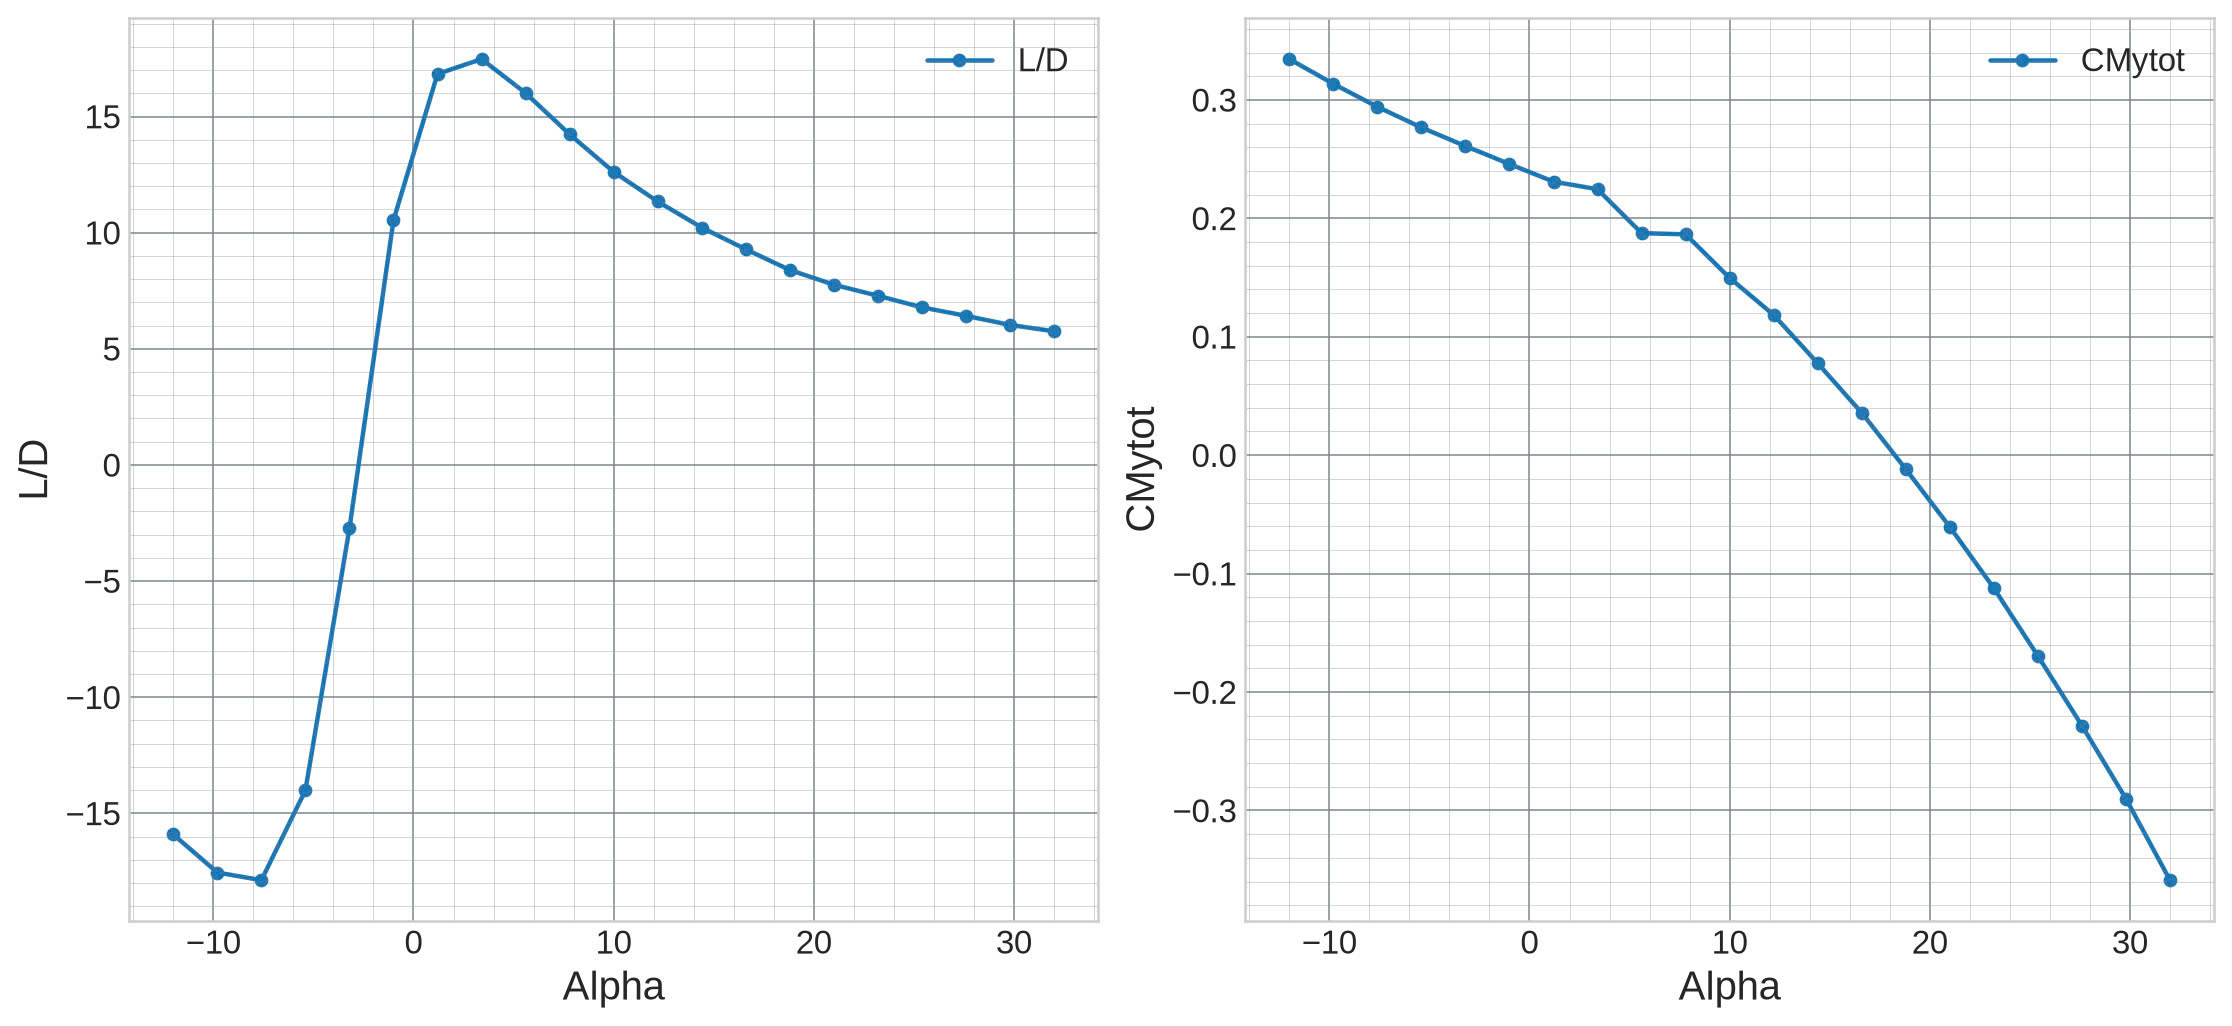
\includegraphics[width=\textwidth]{./images/aerodynamic performance.jpeg}
    \caption{OpenVSP lift-to-drag ratio and pitching-moment coefficient of the full airframe against angle of attack.}
    \label{fig:aero-performance}
\end{figure}

Since $L=C_L(\tfrac12\rho V^2S)$ and $D=C_D(\tfrac12\rho V^2S)$, their ratio is $L/D=C_L/C_D$. The OpenVSP lift-to-drag ratio peaks near \ang{3}--\ang{4} at about 17. Its pitching-moment slope is negative and crosses zero near \ang{19}. Without confirming the moment reference point and trim, this does not establish stability at cruise or validate Gazebo against flight data.

% \textbf{Model check.} Every lift-drag panel of the flown model was ranked by the maximum lift it can make, $S\,C_{L,\max}$ with $C_{L,\max}=C_{L\alpha}\,\alpha_{\mathrm{stall}}$ (Table~\ref{tab:surface-ranking}; left and right panels combined, shares of the wing and horizontal-tail total of \SI{0.428}{\meter\squared}). The script is listed in Appendix~\ref{sec:appendix-names}.



% \begin{table}[H]
% \centering
% \caption{Lifting surfaces of the flown Gazebo model, ranked by maximum lift: the aileron and elevator panels have an unphysical $C_{L,\max}$.}
% \label{tab:surface-ranking}
% \resizebox{\textwidth}{!}{%
% \begin{tabular}{lcccccc}
% \hline
% Surface & $S$ [\si{\meter\squared}] & $C_{L\alpha}$ [\si{\per\radian}] & $\alpha_{\mathrm{stall}}$ & $C_{L,\max}$ & $S\,C_{L,\max}$ [\si{\meter\squared}] & Share \\
% \hline
% Main wing (centre panel) & 0.1832 & 3.70 & \ang{19.4} & 1.25 & 0.230 & \SI{54}{\percent} \\
% Aileron sections (2)     & 0.0177 & 6.80 & \ang{36.6} & \textbf{4.35} & 0.077 & \SI{18}{\percent} \\
% Elevator                 & 0.0155 & 6.80 & \ang{36.6} & \textbf{4.35} & 0.067 & \SI{16}{\percent} \\
% Horizontal tail          & 0.0425 & 3.70 & \ang{19.4} & 1.25 & 0.053 & \SI{12}{\percent} \\
% \hline
% \end{tabular}}
% \end{table}

% Four problems follow from the table and the model file.
% \begin{enumerate}
%     \item \textbf{The wing coefficients are not from OpenVSP.} The main-wing and aileron values ($\alpha_0$, $C_{L\alpha}$, $C_{D\alpha}$, $\alpha_{\mathrm{stall}}$) are identical, to ArduPilot's example Zephyr flying-wing model. Only the areas and centres of pressure were changed, and the areas do match OpenVSP (\SI{0.201}{} against \SI{0.204}{\meter\squared}). OpenVSP gives a lift slope of \SI{5.98}{\per\radian} and a zero-lift offset of \SI{0.049}{\radian}; the model uses 3.70 and 0.130 (Table~\ref{tab:liftdrag-params}).
%     \item \textbf{The aileron and elevator panels are unrealistic.} A lift coefficient of 4.35 at a stall angle of \ang{36.6} is far beyond any plain airfoil (about 1.2--1.6 at \ang{12}--\ang{16}). The elevator, a \SI{0.015}{\meter\squared} strip, can lift more than the whole horizontal tail in front of it, and the two aileron sections add \SI{33}{\percent} to the maximum lift of the wing.
%     \item \textbf{No panel carries a pitching moment} ($C_{m\alpha}=0$ everywhere). The OpenVSP pitching-moment curve is not in the model; pitch stability comes only from where the panels sit.
%     \item \textbf{The weight used earlier was wrong.} The earlier stall estimate used \SI{27.5}{\newton}, which is the fuselage link alone. The model's twelve links total \SI{3.184}{\kilo\gram}, a weight of \SI{31.2}{\newton}.
% \end{enumerate}

% With the correct weight, the 1-g stall speed $V_s=\sqrt{2W/(\rho\,\sum S C_{L,\max})}$ is \SI{15.0}{\meter\per\second} for the centre wing panel alone, \SI{13.0}{\meter\per\second} with the aileron sections, and \SI{11.0}{\meter\per\second} with every horizontal panel. In the calm INDI run the aircraft held \ang{46.9} of bank at \SI{16.75}{\meter\per\second}, which is equivalent to \SI{13.8}{\meter\per\second} in level flight, without stalling. That is below the centre-wing bound. The model can fly there only because of the extra lift of the aileron sections, whose $C_{L,\max}$ is not physical. The \SI{14}{\meter\per\second} minimum airspeed of Section~\ref{sec:mission-profile} is therefore safe in this model but would not be on an aircraft whose outer wing stalls like a real airfoil.

% Two further findings concern the control surfaces. The servo scaling for the rudders gives a travel of only about \ang{0.06}, so the rudders do not move in any run; yaw in wing-borne flight comes from the fins' passive weathercock stability alone. The ailerons and elevator travel $\pm\ang{25}$.

% \textbf{Propellers.} In the model each propeller is two lift-drag panels on a spinning link, so thrust grows with the square of rotor speed, $T_i=k_{T_i}\Omega_i^2$ and $Q_i=k_{Q_i}\Omega_i^2$. The constants are set by the blade panels, not by the bench measurements of Fig.~\ref{fig:stationary-bench}. Yaw moment comes from the difference in rotor drag torque, which is governed by $k_{Q_i}$ and is the least certain part of the propulsion model; this is one reason yaw stays on the PID (Section~\ref{sec:results-yaw}).
% \begin{equation}
%     T_i=k_{T_i}\Omega_i^2,\qquad Q_i=k_{Q_i}\Omega_i^2
%     \label{eq:propeller}
% \end{equation}

% These problems do not affect the PID/INDI comparison directly, because both controllers fly the same model. They do limit how far any simulated result transfers to the real aircraft (Section~\ref{sec:limitations}).

\subsection{Measured control effectiveness}
\label{sec:results-identification}
\label{sec:results-yaw}
The separate test flights described in Section~\ref{sec:identification-method} gave the values in Table~\ref{tab:identification}. The motor values describe hovering flight. The surface values were adjusted to a common reference airspeed of \SI{15}{\meter\per\second} so the three flight speeds could be compared. ``Fit error'' shows how closely the simple response model followed the recorded data; it is \emph{not} an uncertainty bound on $G$. ``Bins'' counts the usable frequency points in each test.

\begin{table}[H]
\centering
\caption{Control effectiveness $G$ measured in simulation, with response lag $\tau$ and delay $T$. Surface values are referred to \SI{15}{\meter\per\second}; yaw is not used by INDI.}
\label{tab:identification}
\begin{tabular}{llcccc}
\hline
Effector & Axis & $G$ [\si{\radian\per\second\squared}] & $\tau$, $T$ [\si{\milli\second}] & Fit error & Bins \\
\hline
Lift motors & roll  & 56.7 & 0, 4 & \SI{11}{\percent} & 118 \\
\hline
            & pitch & 44.8 & 0, 4 & \SI{7}{\percent}  & 116 \\
\hline
            & yaw   & 5.4  & 0, 28 & \SI{45}{\percent} & 53 \\
\hline
Surfaces    & roll  & 16.5--16.8 (3 speeds) & 8--11, $\leq$1 & 8--\SI{21}{\percent} & 49--80 \\
\hline
            & pitch & 12.4--12.5 (3 speeds) & 9--10, 0 & 13--\SI{17}{\percent} & 37--82 \\
\hline
\end{tabular}
\end{table}

The measured motor values are 56.7 for roll and 44.8 for pitch, in \si{\radian\per\second\squared} per unit command. A rough calculation from the simulator's motor positions, thrust and inertia gives 56.9 and 44.8, respectively. The close match is a useful check that the measurements make sense \emph{within the simulator}; it does not check the real aircraft. At three simulated airspeeds near 18.4, 19.9 and \SI{20.8}{\meter\per\second}, the surface values become similar after accounting for the expected $V^2$ change: about 16.5--16.8 for roll and 12.4--12.5 for pitch at the reference speed. The controller therefore uses 16.7 and 12.4 for the surfaces (Appendix~\ref{sec:appendix-parameters}). The yaw test had a much larger fit error (\SI{45}{\percent}), so yaw remains on the stock PID. Only one test flight was made for each flight phase; there are no repeatability bounds, no measurements of coupling between axes and no suitable real forward-flight data. These values are reasonable settings for the \emph{simulated} aircraft, not validated values for the physical one.

\subsection{Simulation checks}
\label{sec:results-wind}
\textbf{Wind.} An aircraft that feels a crosswind must crab. On the long zigzag crosswind legs the mean crab angle matches $\arcsin(W/V_a)$ within \SI{2}{\degree} for both controllers: \SIrange{22.2}{22.8}{\degree} against \SIrange{22.0}{22.4}{\degree} expected at \SI{6}{\meter\per\second}, and \SIrange{35.4}{42.4}{\degree} against \SIrange{35.1}{40.4}{\degree} at \SI{9}{\meter\per\second}. The wind therefore acts on the aerodynamics, not only on the navigation.

\textbf{IMU noise.} For each noisy run, a copy of the Gazebo model adds zero-mean Gaussian noise to every gyro and accelerometer axis at the IMU update rate of \SI{1}{\kilo\hertz}, before ArduPilot's filters. Gazebo IMU sensors report angular velocity and linear acceleration, and its Gaussian-noise model is configured by a mean and standard deviation \citep{gazebosensors,gazebonoise}. The six standard deviations were adjusted using logged post-filter hover spectra until the \SIrange{20}{120}{\hertz} band RMS was close to the real aircraft. Figure~\ref{fig:noisy-imu-validation} compares the real hover with clean and noise-injected simulated hover. In that band, the roll-gyro RMS was \SI{0.251}{\degree\per\second} in simulation versus \SI{0.254}{\degree\per\second} in the aircraft. The clean simulation already had too much pitch-band noise, so adding Gaussian noise could not correct it; its pitch noise remained \SI{74}{\percent} high. This white-noise model does not reproduce the real rotor lines at 53, 71 and \SI{83}{\hertz}. The noise-injected model was used for the comparisons below.

\begin{figure}[H]
    \centering
    \includegraphics[width=0.98\textwidth]{../runs/noisy_wind/imu_match_final.png}
    \caption{Hover gyro spectra: simulated roll noise matches the measured band RMS but not the rotor lines or pitch spectrum.}
    \label{fig:noisy-imu-validation}
\end{figure}

\subsection{Hover torque test}
\label{sec:results-hover-test}
A completed mission does not prove INDI flew it, because the PID remains as a fallback. The aircraft therefore hovered at \SI{20}{\meter} over the origin in the position-hold mode while a constant torque of \SI{1.44}{} or \SI{3.24}{\newton\meter} was applied for \SI{5}{\second} in roll, then in pitch (calm air, IMU noise). Section~\ref{sec:pid-vs-indi-disturbance} predicts the difference: PID must accumulate error in its integrator, INDI corrects at the next step. In the INDI runs the activity flag is set on \SI{100}{\percent} of the samples during every push, and the command steps to its new level within \SI{0.05}{\second}.

\begin{table}[H]
\centering
\caption{Hover torque test, PID / INDI: INDI holds pitch within \SI{0.1}{\degree} and drifts less; the row marked $^\ast$ saturates a lift motor.}
\label{tab:hover-test}
\resizebox{\textwidth}{!}{%
\begin{tabular}{llcccc}
\hline
Torque & Axis & Peak deviation [\si{\degree}] & Held deviation [\si{\degree}] & Distance from origin [\si{\meter}] & Pitch ringing after release [\si{\degree} RMS] \\
\hline
\SI{1.44}{\newton\meter} & roll  & 1.64 / 1.24 & 0.37 / 0.53 & 0.44 / 0.15 & \\
\hline
                         & pitch & 3.26 / 0.79 & 0.81 / 0.04 & 0.90 / 0.09 & 1.68 / 0.14 \\
\hline
\SI{3.24}{\newton\meter} & roll$^\ast$ & 4.02 / 4.10 & 1.53 / 1.50 & 2.05 / 1.08 & \\
\hline
                         & pitch & 7.44 / 1.81 & 2.48 / 0.10 & 2.02 / 0.20 & 3.38 / 0.33 \\
\hline
\end{tabular}}
\end{table}
\begin{figure}[H]
    \centering
    \includegraphics[width=\textwidth]{../runs/hover_test/hover_disturbance.pdf}
    \caption{Hover torque test, pushes shaded: under the pitch torque PID leans, drifts and rings after release, while INDI barely moves.}
    \label{fig:hover-test}
\end{figure}

In Table~\ref{tab:hover-test}, ``held'' is the mean attitude deviation over the final \SI{2}{\second} of each push; distance is the maximum displacement during and shortly after it. Figure~\ref{fig:hover-test} shows the response. For pitch, INDI holds within \SI{0.1}{\degree}, versus \SIrange{0.8}{2.5}{\degree} for PID. At \SI{1.44}{\newton\meter} roll torque, INDI reduces the peak and drift, but PID has the smaller held roll deviation (\ang{0.37} versus \ang{0.53}). At \SI{3.24}{\newton\meter} roll torque, both encounter a motor limit. The command response also differs from that predicted using $G$; command normalisation and mixer effects have not been isolated, so this does not establish a new effectiveness value.

\subsection{PID and INDI comparison}
\label{sec:results-comparison}
Twelve missions were flown (two profiles, two controllers, three conditions, one seed each). All landed; the last-leg midpoint pulse was skipped for INDI on the \SI{9}{\meter\per\second} zigzag after an early landing approach. Table~\ref{tab:summary} summarises these runs; per-pulse peaks and saturation counts are in Appendix~\ref{sec:appendix-results}. An earlier campaign had multiple seeds but different assist conditions, so its spread cannot establish significance for these single runs.

\begin{table}[H]
\centering
\caption{Selected measurements from one PID and one INDI run per case; differences are descriptive, not statistical conclusions.}
\label{tab:summary}
\small
\begin{tabularx}{\textwidth}{>{\raggedright\arraybackslash}p{0.15\textwidth}>{\raggedright\arraybackslash}X>{\centering\arraybackslash}p{0.17\textwidth}>{\centering\arraybackslash}p{0.17\textwidth}>{\raggedright\arraybackslash}p{0.09\textwidth}}
\toprule
Aspect & Measure & PID & INDI & Observed \\
\midrule
Hover, constant torque & pitch, \SI{3.24}{\newton\meter}: held deviation / drift & \SI{2.48}{\degree} / \SI{2.0}{\meter} & \SI{0.10}{\degree} / \SI{0.2}{\meter} & INDI \\
\midrule
 & roll, \SI{1.44}{\newton\meter}: peak / drift & \SI{1.64}{\degree} / \SI{0.44}{\meter} & \SI{1.24}{\degree} / \SI{0.15}{\meter} & INDI \\
\midrule
Hover and transition & take-off pitch RMS & 0.54--\SI{2.03}{\degree} & 0.06--\SI{0.33}{\degree} & INDI \\
\midrule
 & transition pitch RMS & 1.07--\SI{3.34}{\degree} & 0.73--\SI{2.40}{\degree} & INDI \\
\midrule
 & pitch-pulse peak & 2.8--\SI{17.5}{\degree} & 0.8--\SI{10.7}{\degree} & INDI \\
\midrule
Wing-borne & roll-rate tracking RMS, calm & 7.2--\SI{7.3}{\degree\per\second} & 2.0--\SI{2.3}{\degree\per\second} & INDI \\
\midrule
 & roll attitude RMS, calm & 13.5--\SI{15.1}{\degree} & 14.7--\SI{17.9}{\degree} & PID \\
\midrule
 & roll attitude RMS, \SI{6}{\meter\per\second} & 17.1--\SI{17.3}{\degree} & 12.6--\SI{13.2}{\degree} & INDI \\
\midrule
 & pulse peak median, pitch / roll, \SI{6}{\meter\per\second} & 9.8--12.0 / \SIrange{49}{56}{\degree} & 2.9--5.7 / \SIrange{21}{44}{\degree} & INDI \\
\midrule
Path & zigzag straight-leg cross-track, calm / 6 / \SI{9}{\meter\per\second} & 0.95 / 2.5 / \SI{11.9}{\meter} & 1.6 / 1.6 / \SI{3.6}{\meter} & INDI in wind \\
\midrule
 & square height RMS, \SI{6}{\meter\per\second} & \SI{10.5}{\meter} & \SI{2.2}{\meter} & INDI \\
\midrule
\SI{9}{\meter\per\second} limits & wing-borne pulses meeting a saturated effector & 37 of 40 (motors) & 27 of 38 (surfaces) & neither \\
\midrule
 & wing-borne time with lift-motor assist & 72--\SI{83}{\percent} & 0--\SI{9}{\percent} & --- \\
\midrule
 & upsets caught by the lift motors' angle assist & 9 & 4 & --- \\
\bottomrule
\end{tabularx}
\end{table}

\textbf{Shared correction.} Table~\ref{tab:allocation-use} shows how often both effector sets ran INDI together (``both'') and the mean surface share, $G_s^2/(G_m^2+G_s^2)$. During transition, both sets ran INDI together for \SIrange{73}{100}{\percent} of the time. The surfaces supplied about \SI{4}{\percent} of each correction, as Table~\ref{tab:joint-margins} predicts below the \SI{14}{\meter\per\second} transition-end speed. In wing-borne flight, the surfaces supplied all of it.

\begin{table}[H]
\centering
\caption{Use of the shared correction, roll axis: the surfaces take a few per cent of it in the transition and all of it wing-borne.}
\label{tab:allocation-use}
\resizebox{\textwidth}{!}{%
\begin{tabular}{lcccccc}
\hline
 & \multicolumn{2}{c}{Square, calm} & \multicolumn{2}{c}{Square, \SI{9}{\meter\per\second}} & \multicolumn{2}{c}{Zigzag, \SI{6}{\meter\per\second}} \\
Phase & Both & Surface share & Both & Surface share & Both & Surface share \\
\hline
Take-off hover   & \SI{0}{\percent}  & ---                & \SI{81}{\percent}  & \SI{1.1}{\percent} & \SI{0}{\percent}  & --- \\
\hline
Transition       & \SI{73}{\percent} & \SI{4.2}{\percent} & \SI{100}{\percent} & \SI{3.6}{\percent} & \SI{89}{\percent} & \SI{3.8}{\percent} \\
\hline
Wing-borne       & \SI{0}{\percent}  & \SI{100}{\percent} & \SI{0}{\percent}   & \SI{100}{\percent} & \SI{0}{\percent}  & \SI{100}{\percent} \\
\hline
Back-transition  & \SI{96}{\percent} & \SI{9.1}{\percent} & \SI{93}{\percent}  & \SI{13.6}{\percent} & \SI{95}{\percent} & \SI{10.8}{\percent} \\
\hline
Landing hover    & \SI{2}{\percent}  & \SI{0.9}{\percent} & \SI{79}{\percent}  & \SI{2.1}{\percent} & \SI{17}{\percent} & \SI{1.0}{\percent} \\
\hline
\end{tabular}}
\end{table}

\textbf{Attitude and pulses.} In these runs, INDI had lower take-off and transition pitch error (Table~\ref{tab:joint-attitude}) and lower pitch-pulse peaks (Table~\ref{tab:joint-pulses}). Wing-borne roll error was lower at \SI{6}{\meter\per\second} but higher in calm air. Different motor-assist use and one run per case mean the rate controller alone cannot explain every difference.

\begin{table}[H]
\centering
\caption{Attitude tracking error RMS [\si{\degree}], PID / INDI: INDI is lower in take-off and transition in every case.}
\label{tab:joint-attitude}
\resizebox{\textwidth}{!}{%
\begin{tabular}{llcccc}
\hline
Profile & Condition & Take-off pitch & Transition pitch & Wing-borne roll & Landing pitch \\
\hline
Square & calm & 0.54 / 0.06 & 1.10 / 0.77 & 15.1 / 17.9 & 0.58 / 0.30 \\
\hline
       & \SI{6}{\meter\per\second} & 1.46 / 0.33 & 1.40 / 0.94 & 17.3 / 13.2 & 1.31 / 0.40 \\
\hline
       & \SI{9}{\meter\per\second} & 2.02 / 0.32 & 3.34 / 2.40 & 18.2 / 17.0 & 1.79 / 7.01 \\
\hline
Zigzag & calm & 0.54 / 0.06 & 1.07 / 0.73 & 13.5 / 14.7 & 0.46 / 0.30 \\
\hline
       & \SI{6}{\meter\per\second} & 1.44 / 0.33 & 1.21 / 1.00 & 17.1 / 12.6 & 1.49 / 0.92 \\
\hline
       & \SI{9}{\meter\per\second} & 2.03 / 0.32 & 2.99 / 1.29 & 17.0 / 19.3 & 2.25 / 0.61 \\
\hline
\end{tabular}}
\end{table}
\begin{figure}[H]
    \centering
    \includegraphics[width=\textwidth]{../runs/joint/square/compare/timeline_w6.pdf}
    \caption{Attitude error on the square circuit at \SI{6}{\meter\per\second} with \SI{1.44}{\newton\meter} pulses: INDI's pitch error after the pulses is about half PID's.}
    \label{fig:timeline-square}
\end{figure}
\begin{figure}[H]
    \centering
    \includegraphics[width=\textwidth]{../runs/joint/zigzag/compare/timeline_w9.pdf}
    \caption{Attitude error on the zigzag at \SI{9}{\meter\per\second} with \SI{3.24}{\newton\meter} pulses: the wing-borne pulses upset both controllers.}
    \label{fig:timeline-zigzag}
\end{figure}

Both figures plot roll and pitch error on the common clock of Section~\ref{sec:metrics}. Grey bands are \SI{1}{\second} pulses that both runs received, a band in one run's colour a pulse only that run received, and dotted lines the phase changes (T transition start, W wing-borne, B back-transition, L landing hover). On the square at \SI{6}{\meter\per\second} (Fig.~\ref{fig:timeline-square}) INDI halves the median wing-borne pitch peak and lowers the roll peak, while the corners give both controllers large roll errors. On the zigzag at \SI{9}{\meter\per\second} (Fig.~\ref{fig:timeline-zigzag}) the pulses at the turnarounds upset both, with roll errors beyond \SI{140}{\degree}. INDI's last leg there is compressed because it flew the pattern faster and switched to hover early (B), while PID flew most of it slowly with the lift motors assisting; the blue band near \SI{383}{\second} is the last-leg midpoint window, which only PID received.

\textbf{Path.} Corners dominate the wing-borne path error for both controllers: the turn radius carries the aircraft \SIrange{25}{100}{\meter} past them. Table~\ref{tab:joint-path} therefore gives the cross-track RMS on straight legs (points more than \SI{60}{\meter} from a waypoint) separately from the largest cross-track anywhere in wing-borne flight, together with the height RMS on straight legs. On the zigzag's straight legs INDI holds the line better in wind and slightly worse in calm air. On the square's short sides, mostly spent recovering from the previous corner, INDI is worse in every condition.

\begin{table}[H]
\centering
\caption{Wing-borne path error [\si{\meter}], PID / INDI: in wind INDI holds the zigzag's straight legs better; on the square its cross-track error is larger.}
\label{tab:joint-path}
\resizebox{0.9\textwidth}{!}{%
\begin{tabular}{llccc}
\hline
Profile & Condition & Cross-track RMS, straight & Cross-track max & Height RMS, straight \\
\hline
Square & calm & 4.3 / 5.5 & 27 / 32 & 1.4 / 1.7 \\
\hline
       & \SI{6}{\meter\per\second} & 11.0 / 13.1 & 46 / 53 & 10.5 / 2.2 \\
\hline
       & \SI{9}{\meter\per\second} & 16.8 / 27.0 & 54 / 101 & 3.7 / 2.1 \\
\hline
Zigzag & calm & 0.95 / 1.6 & 40 / 43 & 1.1 / 1.3 \\
\hline
       & \SI{6}{\meter\per\second} & 2.5 / 1.6 & 50 / 54 & 1.5 / 1.4 \\
\hline
       & \SI{9}{\meter\per\second} & 11.9 / 3.6 & 50 / 67 & 3.4 / 6.7 \\
\hline
\end{tabular}}
\end{table}

Each row of Figs.~\ref{fig:path-square} and~\ref{fig:path-zigzag} is one condition. The left panel is the flown path over the desired one (top view); the middle and right panels are the signed cross-track error and the height error $e_z$ on the common clock, with the pulses shaded (grey where both runs received the window). Hover phases have no desired height and are left out. The cross-track spikes are the corners and, on the zigzag, the turnarounds, where the \SI{100}{\meter} side step is flown with a \SI{9}{\meter\per\second} tailwind in the strongest case. On the square at \SI{6}{\meter\per\second} PID loses about \SI{10}{\meter} of height for most of the circuit, which also shows as a lower circuit in the 3D view of Fig.~\ref{fig:path-3d}. There the height axis is drawn eight times its true scale, the desired path is dashed and dots mark the pulse starts; the lowest wing-borne points, \SI{16.8}{\meter} (PID, square) and \SI{14.4}{\meter} (INDI, zigzag), both follow upsets at \SI{9}{\meter\per\second}.

\begin{figure}[H]
    \centering
    \includegraphics[width=\textwidth,height=0.4\textheight,keepaspectratio]{../runs/joint/square/path_error/path_square.pdf}
    \caption{Path error on the square circuit: the corners dominate the cross-track error, and PID loses height at \SI{6}{\meter\per\second}.}
    \label{fig:path-square}
    \vspace{0.5\baselineskip}
    \includegraphics[width=\textwidth,height=0.4\textheight,keepaspectratio]{../runs/joint/zigzag/path_error/path_zigzag.pdf}
    \caption{Path error on the zigzag: the turnarounds dominate, and in wind INDI holds the straight legs better.}
    \label{fig:path-zigzag}
\end{figure}

\begin{figure}[H]
    \centering
    \includegraphics[width=\textwidth]{../runs/joint/square/path_error/path3d_square.pdf}
    \includegraphics[width=\textwidth]{../runs/joint/zigzag/path_error/path3d_zigzag.pdf}
    \caption{Whole flights in 3D, square (top) and zigzag (bottom): the largest height losses follow upsets at \SI{9}{\meter\per\second}.}
    \label{fig:path-3d}
\end{figure}

\textbf{Wing-borne comparison.} INDI had smaller roll-rate tracking error in these runs (Table~\ref{tab:summary}), but the rate law alone cannot explain the wing-borne attitude and path differences. Navigation turns, the modelled surface authority and motor assist also matter. PID used assist for \SIrange{72}{83}{\percent} of wing-borne flight, compared with \SIrange{0}{9}{\percent} for INDI. Many \SI{9}{\meter\per\second} pulses reached an effector limit. The Gazebo surface coefficients also differ from the designed aircraft (Section~\ref{sec:aero-model-method}).

Overall, the simulated hover-torque response agrees with INDI's use of measured acceleration (Section~\ref{sec:pid-vs-indi-disturbance}). The shared-correction margins come from the loop model. The wing-borne results also reflect assist and saturation. None of these results proves performance on hardware.

\subsection{Limitations of the study}
\label{sec:limitations}
\begin{itemize}
    \item \textbf{Hardware transfer.} INDI has not flown on hardware. The available real log cannot validate transition or wing-borne effectiveness and lacks measured airspeed for checking the surface gain law.
    \item \textbf{Simulation fidelity.} Borrowed wing and surface coefficients, ineffective rudders and missing panel pitching moments limit the aerodynamic model (Section~\ref{sec:aero-model-method}). The motor uses simulated velocity control without measured hardware spool-up dynamics; its fitted lag is near zero. SITL also uses a different loop rate and gyro filter, and its injected noise misses the real rotor lines.
    \item \textbf{Comparison limits.} PID gains were not retuned to the INDI margin target. One seed was flown per case; PID and INDI used lift-motor assist for different fractions of wing-borne flight. The \SI{9}{\meter\per\second} torque pulses often saturate effectors and are not aerodynamic gusts.
    \item \textbf{Control scope.} Yaw, navigation and altitude remain on ArduPilot. The shared allocation uses last-cycle gains and does not redistribute commands after saturation; surface effectiveness below the measured airspeed range is extrapolated.
\end{itemize}

\subsubsection{Problems encountered during implementation}
\label{sec:filtering-problem}
Most of these were invisible in the flight itself, because every mission still completed.
\begin{itemize}
    \item \textbf{Incomplete synchronisation.} Filtering only the acceleration, then also the command with the same filter, still limit-cycled: the effector lag and the gyro filter were missing from the command path. Matching all three stages (Eq.~\eqref{eq:sync-fix}) removed the oscillation.
    \item \textbf{Surface INDI in the transition.} The first version ran INDI on the lift motors in hover and transition while the surfaces kept their stock PID, and ran surface INDI only in wing-borne flight. Giving the surfaces an independent INDI law in the transition as well would have doubled the correction in the model (Eq.~\eqref{eq:indi-double-correction}). This case was analysed but never flown; the shared correction of Section~\ref{sec:indi-fw-implementation} was flown instead.
    \item \textbf{Wind as a body force.} An early WindEffects configuration added excessive direct body drag and stopped the transition. Its body-force term was set to zero; the plugin still generates wind and turbulence for the aerodynamic panels.
    \item \textbf{Lost first pulse.} The torque helper sent its first command before Gazebo's messaging had connected, so the first pulse of every run was silently dropped. It now waits for the connection; all disturbed missions were re-flown.
    \item \textbf{Diagnosing the plant as the controller.} A \SI{16}{\hertz} line in the INDI acceleration estimate was taken for a limit cycle until the same line appeared in the PID runs' gyro. A diagnostic computed only inside the controller under test cannot separate controller from plant.
\end{itemize}

\section{Conclusion and Future Work}
\label{sec:conclusion}
The first objective was met in SITL: a synchronized INDI roll-and-pitch rate loop was implemented in ArduPilot, with one correction shared between lift motors and control surfaces and a PID fallback. The discrete loop model predicts that sharing preserves margins; independent full corrections were not flight-tested.

The simulated pitch-torque test shows smaller held error with INDI, and the twelve mission runs show lower recorded take-off and transition pitch errors. The third objective was only partly met: these are comparisons within a simplified Gazebo model, not a validated representation of the real aircraft. One seed, unmatched PID tuning, differing lift-motor assist and saturation prevent a general wing-borne performance claim. The real log provides a warning about hardware gyro noise, not validation of hardware INDI.

\subsection{Future work}
\label{sec:future-work}
\begin{itemize}
    \item Match aerodynamic coefficients, rotor and servo dynamics, and gyro settings to hardware; measure airspeed before using surface INDI on the real aircraft.
    \item Retune the PID baseline, compare matched-assist flight segments, and repeat with several seeds and non-saturating disturbances.
    \item Re-identify effectiveness after model changes; flight-test INDI only after bench and low-altitude safety checks with PID fallback.
\end{itemize}

\bibliographystyle{unsrtnat}
\bibliography{thesis}

\appendix
\section{Physical Prototype Build}
\label{sec:appendix-build}
\begin{figure}[H]
    \centering
    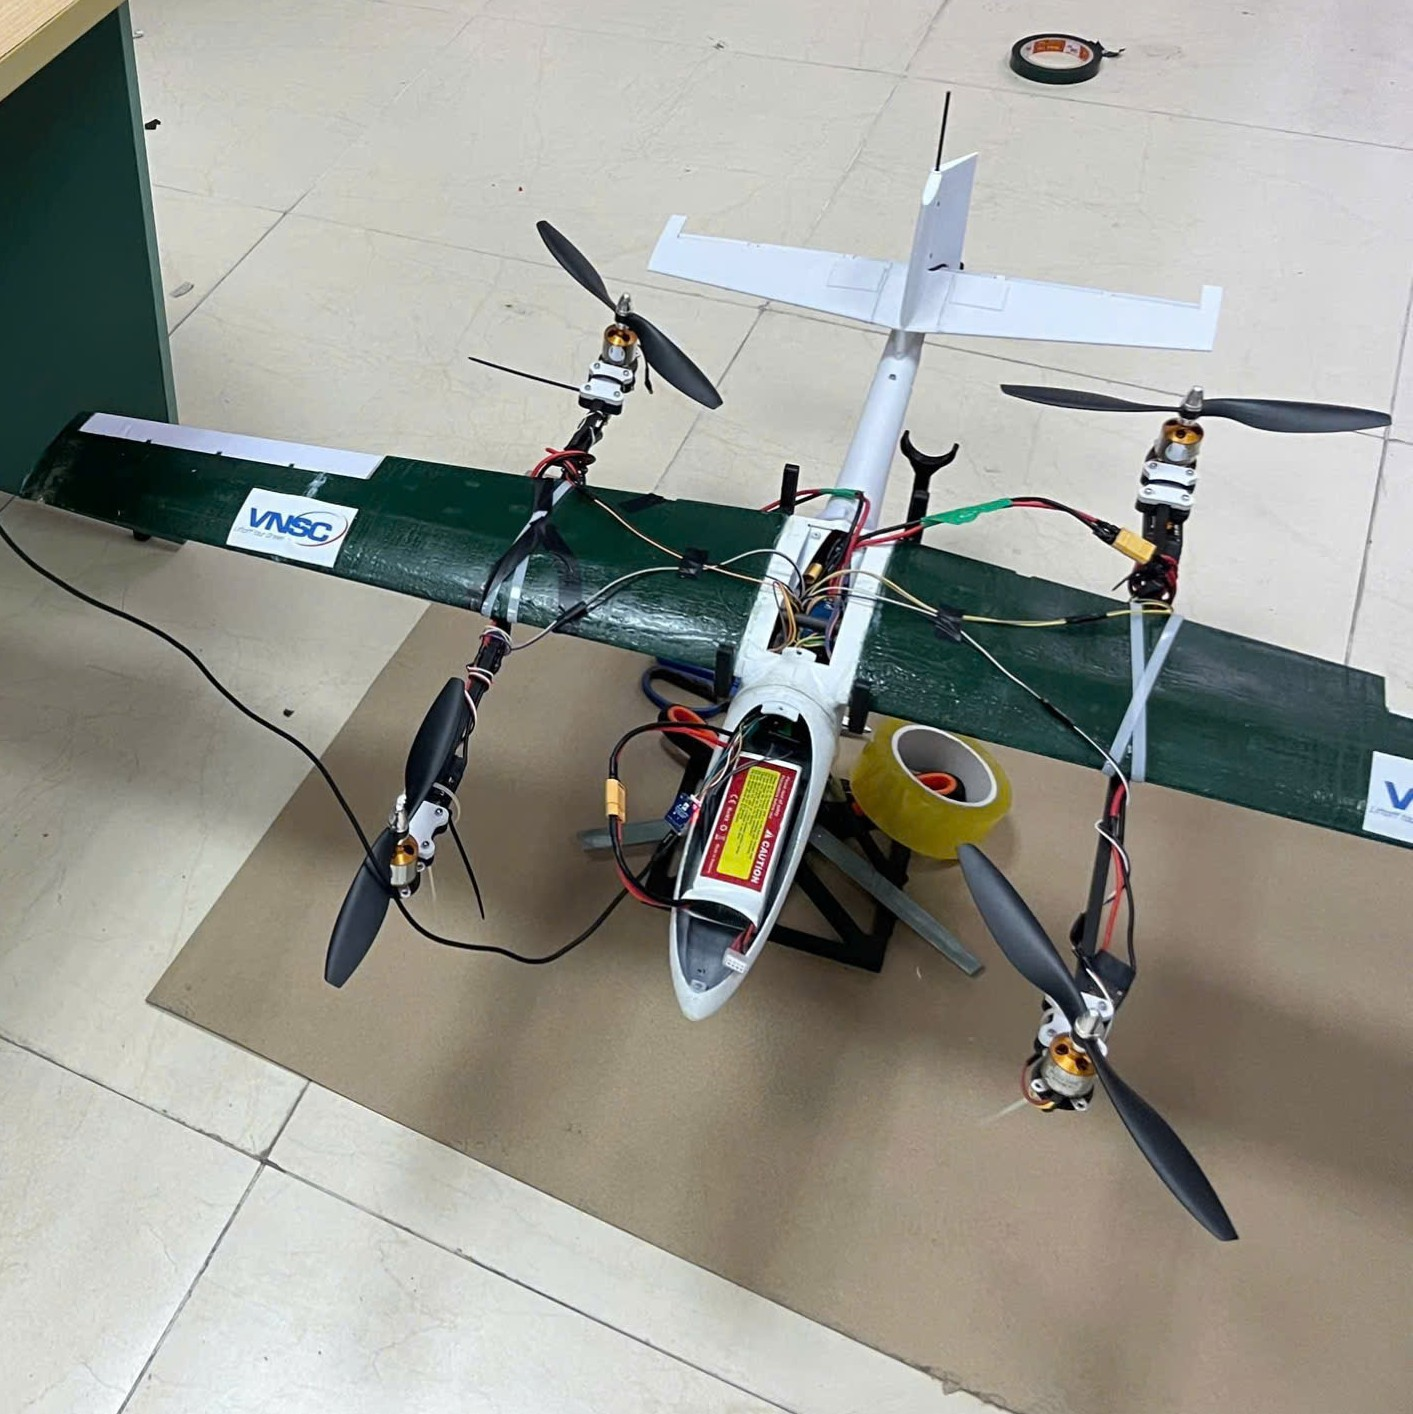
\includegraphics[width=0.85\textwidth,height=0.8\textheight,keepaspectratio]{./images/1st iteration.jpeg}
    \caption{First 3D-printed structural iteration of the wing, boom, and tail assembly, prior to final assembly and avionics integration.}
    \label{fig:first-iteration}
\end{figure}

\begin{figure}[H]
    \centering
    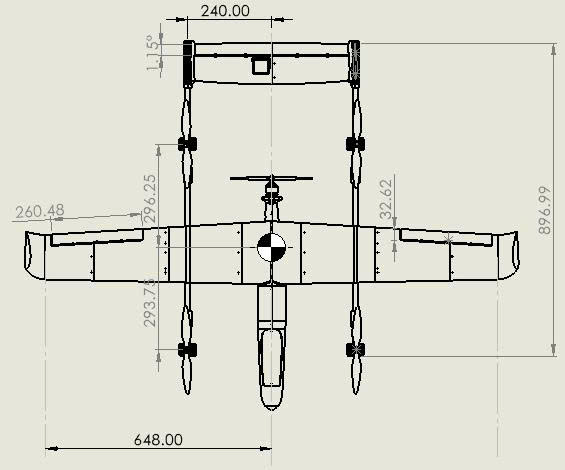
\includegraphics[width=0.82\textwidth,height=0.67\textheight,keepaspectratio]{./images/dimensions1.jpeg}
    \caption{Top view of the CAD airframe of final design (dimensions in mm): wing, four lift-motor positions on the twin booms and the tail.}
    \label{fig:aircraft-dimensions-top}
\end{figure}

\begin{figure}[H]
    \centering
    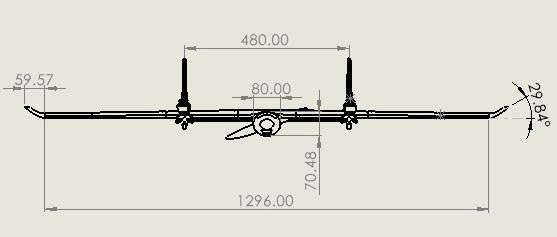
\includegraphics[width=0.94\textwidth,height=0.52\textheight,keepaspectratio]{./images/dimensions2.jpeg}
    \caption{Front view (dimensions in mm).}
    \label{fig:aircraft-dimensions-front}
\end{figure}

\begin{figure}[H]
    \centering
    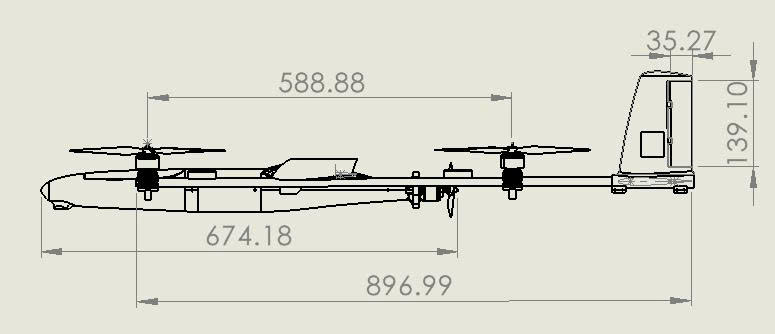
\includegraphics[width=0.94\textwidth,height=0.52\textheight,keepaspectratio]{./images/dimensions3.jpeg}
    \caption{Left-side view (dimensions in mm).}
    \label{fig:aircraft-dimensions-left}
\end{figure}

\section{Additional PID and INDI Results}
\label{sec:appendix-results}
\begin{figure}[H]
    \centering
    \includegraphics[width=\textwidth]{../runs/hover_test/hover_path3d.pdf}
    \caption{Hover-torque test trajectories for PID and INDI. Each panel shows the displacement from the hover origin at one applied torque; dots mark the starts of the \SI{5}{\second} roll and pitch pushes.}
    \label{fig:hover-torque-path3d}
\end{figure}

\begin{figure}[H]
    \centering
    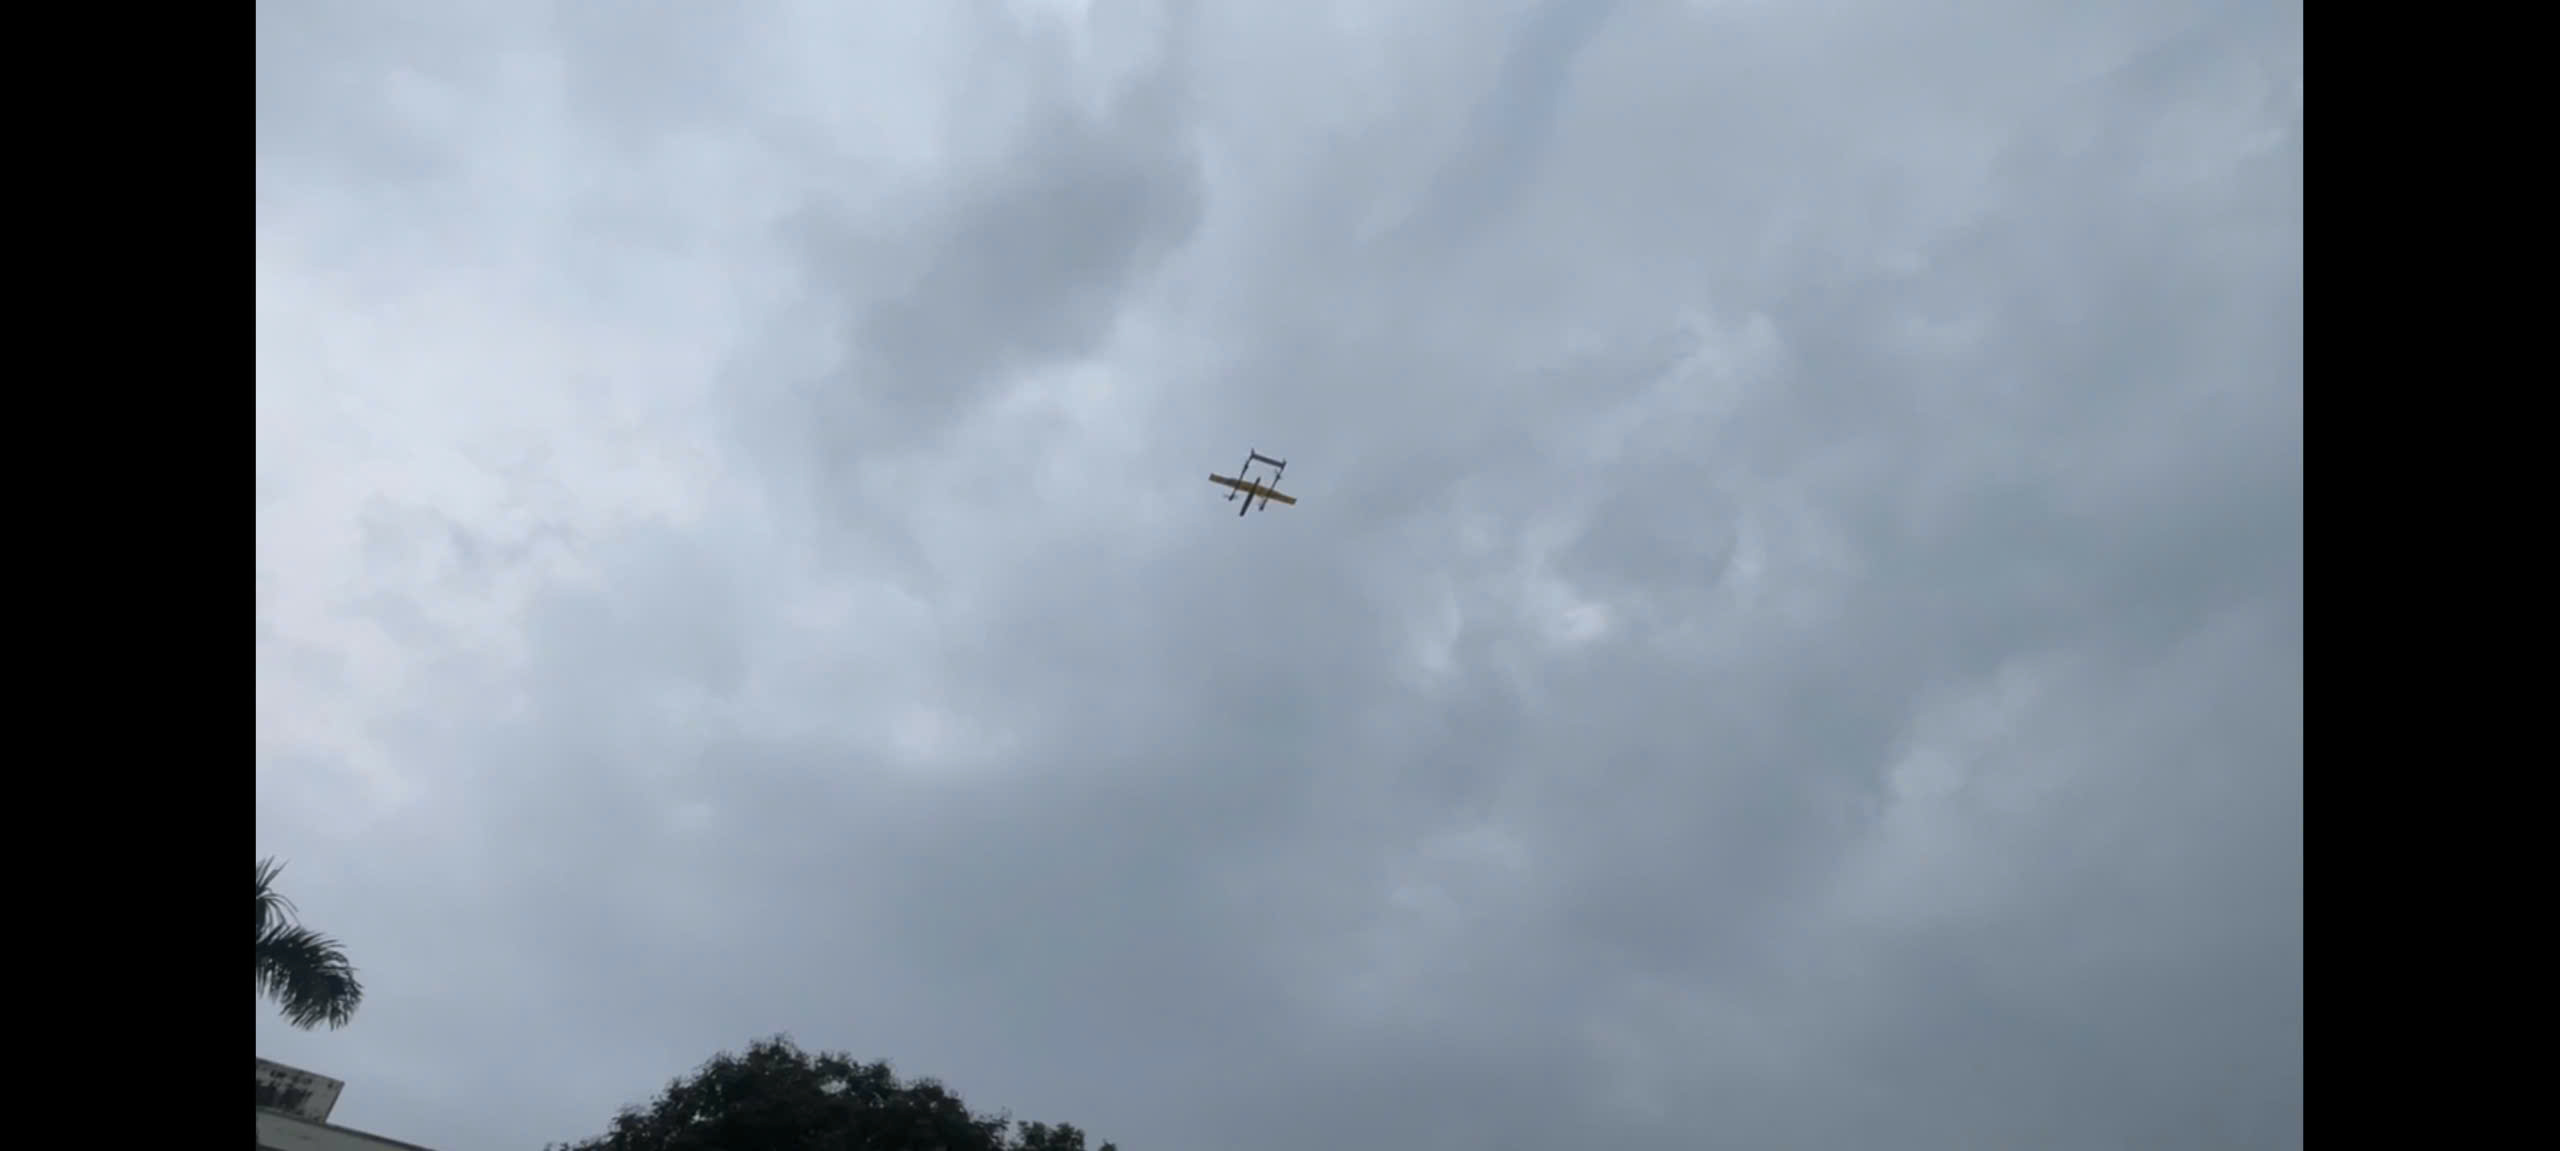
\includegraphics[width=0.72\textwidth,height=0.72\textheight,keepaspectratio]{./images/Real_flight_Hovering.jpeg}
    \caption{Physical prototype during the available real-flight hover. This flight used the stock PID controller; it is not an INDI flight result.}
    \label{fig:real-hover-photo}
\end{figure}

Table~\ref{tab:joint-pulses} gives the peak attitude error after each moment pulse. The hover and transition columns give the range over the take-off, transition and landing windows; the wing-borne columns give the median over the corner and midpoint windows, with the maximum in brackets (square 7 windows, zigzag 12--13).

\begin{table}[H]
\centering
\caption{Peak attitude error after a moment pulse [\si{\degree}], PID / INDI: INDI's hover and transition pitch peaks are smaller in every case.}
\label{tab:joint-pulses}
\resizebox{\textwidth}{!}{%
\begin{tabular}{llcccc}
\hline
Profile & Condition & Hover/transition pitch & Hover/transition roll & Wing-borne pitch & Wing-borne roll \\
\hline
Square & \SI{6}{\meter\per\second} & 3.2--4.8 / 0.8--1.1 & 1.8--5.5 / 1.3--3.9 & 12.0 (20.6) / 5.7 (14.0) & 56 (61) / 21 (45) \\
\hline
       & \SI{9}{\meter\per\second} & 6.7--17.5 / 1.7--10.7 & 4.7--11.8 / 3.2--6.8 & 15.5 (19.2) / 6.3 (15.3) & 37 (143) / 40 (64) \\
\hline
Zigzag & \SI{6}{\meter\per\second} & 2.8--4.9 / 0.8--1.1 & 1.7--4.3 / 1.5--2.5 & 9.8 (21.8) / 2.9 (6.8) & 49 (139) / 44 (95) \\
\hline
       & \SI{9}{\meter\per\second} & 6.8--16.2 / 1.3--6.1 & 4.7--7.9 / 3.3--28.5 & 9.9 (25.0) / 12.8 (23.3) & 112 (164) / 65 (175) \\
\hline
\end{tabular}}
\end{table}

Table~\ref{tab:saturation} counts the pulses that met a saturated effector within \SI{2}{\second} of their start: ``motor limit'' is a lift motor at its minimum or maximum, ``surface'' the pulsed axis' surface at full travel. At \SI{6}{\meter\per\second} saturation is rare. At \SI{9}{\meter\per\second} every hover, transition and landing roll pulse met a lift motor at its limit, for both controllers; wing-borne, PID's pulses met motors at a limit and INDI's met saturated surfaces.

\begin{table}[H]
\centering
\caption{Pulses that met a saturated effector, PID / INDI: at \SI{9}{\meter\per\second} PID meets motor limits and INDI surface limits.}
\label{tab:saturation}
\resizebox{\textwidth}{!}{%
\begin{tabular}{llccccc}
\hline
Profile & Condition & \multicolumn{2}{c}{Hover and transition (6 pulses)} & \multicolumn{3}{c}{Wing-borne} \\
 & & Motor limit & Surface & Pulses & Motor limit & Surface \\
\hline
Square & \SI{6}{\meter\per\second} & 2 / 2 & 0 / 0 & 14 / 14 & 1 / 1 & 0 / 0 \\
\hline
       & \SI{9}{\meter\per\second} & 5 / 5 & 1 / 0 & 14 / 14 & 13 / 0 & 3 / 10 \\
\hline
Zigzag & \SI{6}{\meter\per\second} & 3 / 2 & 0 / 0 & 26 / 26 & 0 / 0 & 0 / 0 \\
\hline
       & \SI{9}{\meter\per\second} & 5 / 6 & 1 / 0 & 26 / 24 & 24 / 8 & 10 / 17 \\
\hline
\end{tabular}}
\end{table}

Figure~\ref{fig:saturation} shows where this happens on the zigzag at \SI{9}{\meter\per\second}, on the common clock with the pulses shaded. The top two rows are the four lift motors of each run (band from the lowest to the highest, line the mean), with the spin limits dashed and red ticks where a motor is at a limit; the rows below are the aileron, elevator and pusher throttle. PID's lift motors run through most of the wing-borne flight because of assist, while INDI's run only in short bursts after an upset.

\begin{figure}[H]
    \centering
    \includegraphics[width=\textwidth]{../runs/joint/zigzag/saturation/saturation_w9.pdf}
    \caption{Effector use on the zigzag at \SI{9}{\meter\per\second}: PID leans on its lift motors, INDI's ailerons reach full travel at the pulses.}
    \label{fig:saturation}
\end{figure}

\section{Vehicle and Controller Parameters}
\label{sec:appendix-parameters}
The PID runs use \texttt{stock\_\allowbreak{}pid.param}. The INDI runs use the same file with \texttt{indi.param} appended, so the two differ only in the lines of Table~\ref{tab:appendix-indi-params}. With \texttt{Q\_INDI\_ENABLE}\,=\,0 (the default) the INDI code is not loaded and the aircraft runs stock ArduPilot.

\begin{table}[H]
    \centering
    \caption{INDI parameters, as flown (\texttt{indi.param}).}
    \label{tab:appendix-indi-params}
    \resizebox{\textwidth}{!}{%
\begin{tabular}{llll}
        \toprule
        Parameter & Value & Source & Role \\
        \midrule
        \texttt{Q\_INDI\_ENABLE}   & 1 & --- & Load the INDI controller at boot \\
        \midrule
        \texttt{Q\_INDI\_AXES}     & 27 & --- & Bitmask: VTOL roll, VTOL pitch, FW roll, FW pitch \\
        \midrule
        \texttt{Q\_INDI\_FILT\_HZ} & \SI{12.7}{\hertz} & design & Two poles of $H$ (Eq.~\eqref{eq:diagonal-inversion}) \\
        \midrule
        \texttt{Q\_INDI\_RLL\_G}   & 56.7 & identified & Lift-motor roll effectiveness \\
        \midrule
        \texttt{Q\_INDI\_PIT\_G}   & 44.8 & identified & Lift-motor pitch effectiveness \\
        \midrule
        \texttt{Q\_INDI\_YAW\_G}   & 0    & excluded   & Zero keeps yaw on the PID \\
        \midrule
        \texttt{Q\_INDI\_ACT\_TC}  & 0    & identified & Lift-motor lag \\
        \midrule
        \texttt{Q\_INDI\_ACT\_DLY} & \SI{4}{\milli\second} & identified & Lift-motor delay \\
        \midrule
        \texttt{Q\_INDI\_RLL\_K}, \texttt{PIT\_K} & \SI{13.5}{\per\second} & margins & Rate error to $\nu$ \\
        \midrule
        \texttt{Q\_INDI\_FW\_RLL\_G} & 16.7 & identified & Aileron effectiveness at \texttt{SCALING\_SPEED} \\
        \midrule
        \texttt{Q\_INDI\_FW\_PIT\_G} & 12.4 & identified & Elevator effectiveness at \texttt{SCALING\_SPEED} \\
        \midrule
        \texttt{Q\_INDI\_FW\_TC}     & \SI{10}{\milli\second} & identified & Surface servo lag \\
        \midrule
        \texttt{Q\_INDI\_FW\_RLL\_K}, \texttt{FW\_PIT\_K} & \SI{10.5}{\per\second} & margins & Rate error to $\nu$ \\
        \bottomrule
    \end{tabular}}
\end{table}

Effectiveness is in \si{\radian\per\second\squared} per unit normalised command: full mixer input for the lift motors, full surface travel for the surfaces. \texttt{SCALING\_SPEED} is \SI{15}{\meter\per\second}; the surface values are multiplied by $(V/\texttt{SCALING\_SPEED})^2$ with the measured airspeed $V$, which is Eq.~\eqref{eq:fw-indi-scaling}. ``Identified'' values come from \texttt{identify\_\allowbreak{}G.py} on the hover and fixed-wing system-identification runs; ``margins'' are the largest gains with at least \SI{6}{\decibel} gain margin and \ang{45} phase margin from \texttt{indi\_\allowbreak{}margins.py}, reduced slightly.
% NOTE 2026-09-26: Section sec:results-identification still quotes G = 61.7 / 55.4 and
% tau = 23 ms from an earlier identification; the flown file uses 56.7 / 44.8, tau 0,
% delay 4 ms. Reconcile the Results text with the identification that produced indi.param.

\begin{table}[H]
    \centering
    \caption{Other settings referred to in the text, as flown (\texttt{stock\_\allowbreak{}pid.param}).}
    \label{tab:appendix-other-params}
    \resizebox{\textwidth}{!}{%
\begin{tabular}{lll}
        \toprule
        Parameter & Value & Plain name in the text \\
        \midrule
        \texttt{AIRSPEED\_STALL}  & \SI{12}{\meter\per\second} & stall speed \\
        \midrule
        \texttt{AIRSPEED\_MIN}    & \SI{14}{\meter\per\second} & minimum airspeed \\
        \midrule
        \texttt{AIRSPEED\_CRUISE} & \SI{17}{\meter\per\second} & cruise airspeed \\
        \midrule
        \texttt{Q\_ASSIST\_SPEED} & \SI{13}{\meter\per\second} & lift-motor assist speed \\
        \midrule
        \texttt{Q\_OPTIONS}       & 0 (bit 7 cleared) & forced-assist setting (bit 7, \texttt{Q\_ASSIST\_FORCE\_ENABLE}) \\
        \midrule
        \texttt{Q\_TRANSITION\_MS} & \SI{3000}{\milli\second} & timed part of the forward transition \\
        \midrule
        \texttt{SCHED\_LOOP\_RATE} & \SI{400}{\hertz} & nominal control-loop rate \\
        \midrule
        \texttt{INS\_GYRO\_FILTER} & \SI{20}{\hertz} & gyro low-pass filter ($F_g$) \\
        \midrule
        \texttt{WP\_RADIUS}       & \SI{25}{\meter} & waypoint acceptance radius \\
        \midrule
        \texttt{NAVL1\_PERIOD}    & \SI{12}{\second} & navigation look-ahead period \\
        \bottomrule
    \end{tabular}}
\end{table}

\section{Names Used in ArduPilot, Gazebo and the Project Files}
\label{sec:appendix-names}
The main text uses plain names. This appendix gives the matching name in the code, the model file or the log.

\begin{longtable}{p{0.40\textwidth}p{0.52\textwidth}}
\textbf{Plain name in the text} & \textbf{Name in ArduPilot, Gazebo or the project files} \\
\midrule
\multicolumn{2}{l}{\emph{Flight modes and log messages}} \\
\midrule
hover mode & \texttt{QHOVER} \\
\midrule
stabilised fixed-wing mode & \texttt{FBWA} \\
\midrule
logged airspeed & \texttt{CTUN.As} \\
\midrule
airspeed-sensor messages & \texttt{ARSP} \\
\midrule
stored hover throttle & \texttt{Q\_M\_THST\_HOVER} \\
\midrule
batch-sampled gyro log & \texttt{INS\_\allowbreak{}LOG\_\allowbreak{}BAT\_\allowbreak{}MASK} \\
\midrule
logged vibration levels & \texttt{VIBE.VibeX/Y/Z} \\
\midrule
logged body rates & \texttt{RATE} \\
\midrule
parameters written at boot & \texttt{PARM} \\
\midrule
INDI log, lift motors / surfaces & \texttt{INDI} \\
\midrule
\multicolumn{2}{l}{\emph{Controller code (branch \texttt{indi})}} \\
\midrule
state estimator & \texttt{EKF3} (\texttt{AP\_NavEKF3}) \\
\midrule
INDI core, one per axis & \texttt{AC\_INDI\_Axis} (\texttt{AC\_INDI.cpp}) \\
\midrule
INDI parameter block & \texttt{AC\_INDI\_Params}, parameters \texttt{Q\_INDI\_*} \\
\midrule
lift-motor INDI rate loop & \texttt{AC\_\allowbreak{}AttitudeControl\_\allowbreak{}INDI::\allowbreak{}rate\_\allowbreak{}controller\_\allowbreak{}run\_\allowbreak{}dt()}, derived from \texttt{AC\_\allowbreak{}AttitudeControl\_\allowbreak{}TS} \\
\midrule
surface INDI rate loop & \texttt{AP\_\allowbreak{}FW\_\allowbreak{}Controller::\allowbreak{}run\_\allowbreak{}rate\_\allowbreak{}control()} \\
\midrule
boot-time switch & \texttt{QuadPlane::setup()} reading \texttt{Q\_INDI\_ENABLE} \\
\midrule
applied mixer input $u_{\mathrm{applied}}$ & \texttt{AC\_\allowbreak{}AttitudeControl\_\allowbreak{}INDI::\allowbreak{}applied\_\allowbreak{}input()} \\
\midrule
\multicolumn{2}{l}{\emph{Gazebo model (\texttt{model.sdf})}} \\
\midrule
lift-drag system & \texttt{gz-sim-lift-drag-system} \\
\midrule
$S$, $\alpha_0$, $C_{L\alpha}$, $C_{D\alpha}$, $C_{m\alpha}$ & \texttt{area}, \texttt{a0}, \texttt{cla}, \texttt{cda}, \texttt{cma} \\
\midrule
$\alpha_{\mathrm{stall}}$, post-stall slopes & \texttt{alpha\_stall}, \texttt{cla\_stall}, \texttt{cda\_stall}, \texttt{cma\_stall} \\
\midrule
$\mathbf{r}_{cp}$, $\hat{\mathbf{e}}_f$, $\hat{\mathbf{e}}_u$ & \texttt{cp}, \texttt{forward}, \texttt{upward} \\
\midrule
$k_\delta$ & \texttt{control\_\allowbreak{}joint\_\allowbreak{}rad\_\allowbreak{}to\_\allowbreak{}cl} \\
\midrule
servo scaling & \texttt{ArduPilotPlugin} \texttt{<multiplier>}, \texttt{<offset>} \\
\midrule
Gazebo wind plugin & \texttt{WindEffects}, links with \texttt{enable\_wind} \\
\midrule
\multicolumn{2}{l}{\emph{Files and scripts}} \\
\midrule
square mission & \texttt{square.plan} \\
\midrule
zigzag mission & \texttt{Default square zigzag path.plan} \\
\midrule
mission runner, pulse schedule & \texttt{fly\_\allowbreak{}plan\_\allowbreak{}mission.py} (class \texttt{Disturbance}) \\
\midrule
torque injection & \texttt{disturb.py} \\
\midrule
lifting-surface ranking & \texttt{rank\_\allowbreak{}lifting\_\allowbreak{}surfaces.py} \\
\midrule
mission geometry & \texttt{plan\_\allowbreak{}geometry.py} \\
\midrule
autopilot stored memory & \texttt{eeprom.bin} \\
\end{longtable}

\section{Gazebo Aerodynamic Model Values}
\label{sec:appendix-config}
\begin{figure}[H]
    \centering
    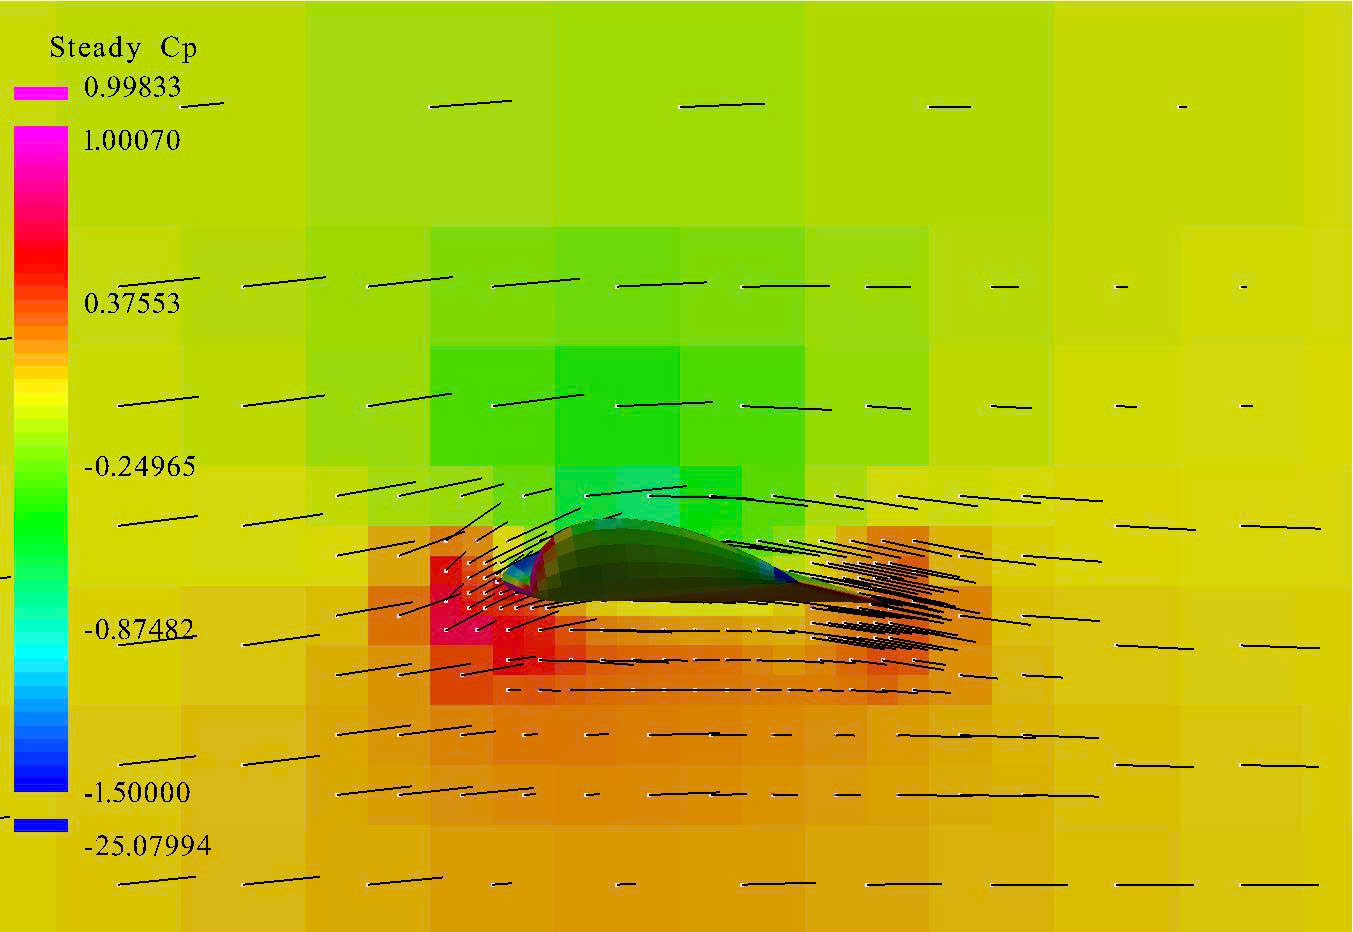
\includegraphics[width=0.7\textwidth]{./images/wing lift vector field.jpeg}
    \caption{OpenVSP pressure coefficient and flow vectors near the fuselage/wing junction.}
    \label{fig:wing-vector-field}
\end{figure}

Table~\ref{tab:liftdrag-params} records the main-wing lift-drag parameters used in the flown Gazebo model, alongside the matching OpenVSP values where available.

\begin{table}[H]
\centering
\caption{Gazebo lift-drag panel parameters: main wing of the flown model against OpenVSP.}
\label{tab:liftdrag-params}
\resizebox{\textwidth}{!}{%
\begin{tabular}{llcc}
\hline
Symbol & Meaning & Main wing (flown) & OpenVSP \\
\hline
$S$ & panel area & \SI{0.183}{\meter\squared} & \SI{0.204}{\meter\squared} (whole wing) \\
\hline
$\alpha_0$ & angle added to the geometric angle of attack & \SI{0.130}{\radian} & \SI{0.049}{\radian} \\
\hline
$C_{L\alpha}$ & lift-curve slope & \SI{3.70}{\per\radian} & \SI{5.98}{\per\radian} \\
\hline
$C_{D\alpha}$ & drag-curve slope & \SI{0.064}{\per\radian} & --- \\
\hline
$C_{m\alpha}$ & pitching-moment slope & 0 & from $C_m(\alpha)$ sweep \\
\hline
$\alpha_{\mathrm{stall}}$ & stall angle & \SI{0.339}{\radian} (\ang{19.4}) & not modelled \\
\hline
$C_{L\alpha,\mathrm{stall}}$ & lift slope after stall & \SI{-3.85}{\per\radian} & not modelled \\
\hline
$C_{D\alpha,\mathrm{stall}}$ & drag slope after stall & \SI{-0.92}{\per\radian} & not modelled \\
\hline
$\mathbf{r}_{cp}$ & centre of pressure, body frame & (0.061, 0, 0.004) \si{\meter} & --- \\
\hline
$\hat{\mathbf{e}}_f,\hat{\mathbf{e}}_u$ & panel forward and upward axes & $+x$, $+z$ & --- \\
\hline
$k_\delta$ & lift coefficient per radian of deflection & --- (ailerons, elevator: $-5$) & --- \\
\hline
\end{tabular}}
\end{table}

\end{document}
